\chapter{Teori}
\label{chap:teori}

\section{Pulsoximetri}
Pulsoximetri er en ikke-invasiv målemetode til bestemmelse af iltmætningen i arterielt blod. Metoden udnytter forskelle i lysabsorption mellem iltet hæmoglobin ($\text{HbO}_2$) og uiltet hæmoglobin ($\text{Hb}$) ved to forskellige bølgelængder af lys, typisk \SI{660}{nm} (rød) og \SI{940}{nm} (nær infrarød). Da målingen oftest foretages perifert, f.eks.\ på fingeren, betegnes resultatet $\text{SpO}_2$, og repræsenterer ikke nødvendigvis iltmætningen i hele kredsløbet. Det er derfor nødvendigt at skelne mellem flere kliniske parametre af ilt \cite{Webster1997,Nitzan2014}.

Hæmoglobin er det iltbærende protein i de røde blodlegemer. Hvert hæmoglobinmolekyle indeholder fire hæmgrupper, som hver kan binde et iltmolekyle reversibelt. Når ilt er bundet, betegnes molekylet oxyhæmoglobin ($\text{HbO}_2$), mens hæmoglobin uden bundet ilt betegnes deoxyhæmoglobin eller uiltet hæmoglobin ($\text{Hb}$). Det er forskellen i disse to formers absorption af lys, der gør pulsoximetri mulig \cite{Webster1997,Nitzan2014}.

\subsection{Kliniske ilt-parametre}
Herunder er en oversigt over de vigtigste kliniske iltparametre \cite{Pltz1998,Nitzan2014,Webster1997,YossefHay2018}:

\begin{description}
    \item[$\text{PaO}_2$ - Partialtryk af ilt i arterielt blod] \hfill
    \\
    Måles direkte med blodgasanalyse. \\
    Enhed: mmHg eller kPa. \\
    Normal: \SI{80}{mmHg} til \SI{100}{mmHg} (\SI{11}{kPa} til \SI{13}{kPa}).

    \item[$\text{SaO}_2$ - Arteriel iltmætning] \hfill
    \\
    Beskriver andelen af hæmoglobin bundet til ilt i arterielt blod. \\
    Måles med blodgasanalyse.  \\
    Enhed: \%.  \\
    Normal: ca.\ 94--98\,\% for raske voksne ved havniveau.

    \item[$\text{CaO}_2$ - Arterielt iltindhold] \hfill
    \\
    Det totale iltindhold i arterielt blod. \\
    Enhed: $\frac{\text{mL\,O}_2}{\text{dL\,blod}}$. \\
    Normal: ca.\ \SI{20}{mL\,O_2/dL}. \\
    Beregnes ud fra \cite[s.~2]{Pltz1998}:
    \begin{equation}
        \text{CaO}_2 = 1.36 \cdot [\text{Hb}] \cdot \text{SaO}_2 + 0.0031 \cdot \text{PaO}_2
        \label{eq:cao2}
    \end{equation}
    Hvor: \\
    $[\text{Hb}]$ er hæmoglobinkoncentrationen i $\frac{\text{g}}{\text{dL}}$ \\
    Konstanten \SI{1.36}{\frac{mL O_2}{g\ Hb}} er iltbindingskapaciteten per gram hæmoglobin \\
    Leddet $0.0031 \cdot \text{PaO}_2$ repræsenterer opløst ilt i plasma (ubetydeligt bidrag).

    \item[$\text{SpO}_2$ - Perifer iltmætning] \hfill
    \\
    Estimat af $\text{SaO}_2$ målt ikke-invasivt med pulsoximeter via lysabsorption
    ved to bølgelængder (f.eks.\ \SI{660}{nm} og \SI{940}{nm}). \\
    Enhed: \%. \\
    Normal: $>$\,95\%. \\
    Denne parameter er fokus for bachelorprojektet.

\end{description}

Blandt disse parametre betragtes $\text{SaO}_2$ som guldstandarden, idet den bestemmes præcist via blodgasanalyse. Blodgasanalyser kræver imidlertid en arteriel blodprøve med en kanyle ind i en arterie og er derfor invasive. \\ 
$\text{SpO}_2$ er et ikke-invasivt estimat af $\text{SaO}_2$, som tillader kontinuerlig måling og er tilgængeligt til en lav pris i flere forbruger og kliniske produkter. Hos kritisk syge voksne patienter kan forskellen mellem $\text{SpO}_2$ og $\text{SaO}_2$ dog være flere procentpoint, hvilket understreger at pulsoximetri ikke er identisk med blodgasbestemt arteriel iltmætning \cite[s.~2]{YossefHay2018}. Den reducerede præcision opvejes af de praktiske fordele ved metoden, dog har begge produkter hver deres plads under udredning og overvågning af sundhed hos mennesker i hjem og hospital.

\subsection{Det fotoplethysmografiske signal}

En plethysmograf er et instrument der måler volumenændringer i et organ, og det resulterende signal kaldes et plethysmogram. Når målingen foregår optisk via lystransmission, betegnes signalet et 
fotoplethysmogram (PPG) \cite{Allen2007}.

Ved måling af lystransmission gennem en finger observeres et periodisk signal der følger hjertets cyklus. Under systole, som er hjertemuskulaturens kontraktion, udvides arterierne og blodvolumen i fingeren forøges, hvilket øger absorptionen og reducerer den transmitterede intensitet. Under diastole, som er fasen med hjertemuskulaturens afslapning, falder blodvolumen og intensiteten stiger igen.

Som set i figur \ref{fig:ppg_signal} \cite{YossefHay2018}, kan PPG signalet opdeles i en DC komponent og en AC komponent. DC komponenten repræsenterer den konstante absorption fra venøst blod, væv, knogle og ikke pulsatilt arterielt og venøst blod. AC komponenten repræsenterer den pulsatile ændring i arterielt blodvolumen og udgør typisk kun få procent af det samlede signal, omkring 1--2\% i klassiske beskrivelser \cite[s.~47]{Webster1997}. Det pulsatile (AC) signal er signalet som PPG måler på.

\begin{figure}[htbp]
     \centering
     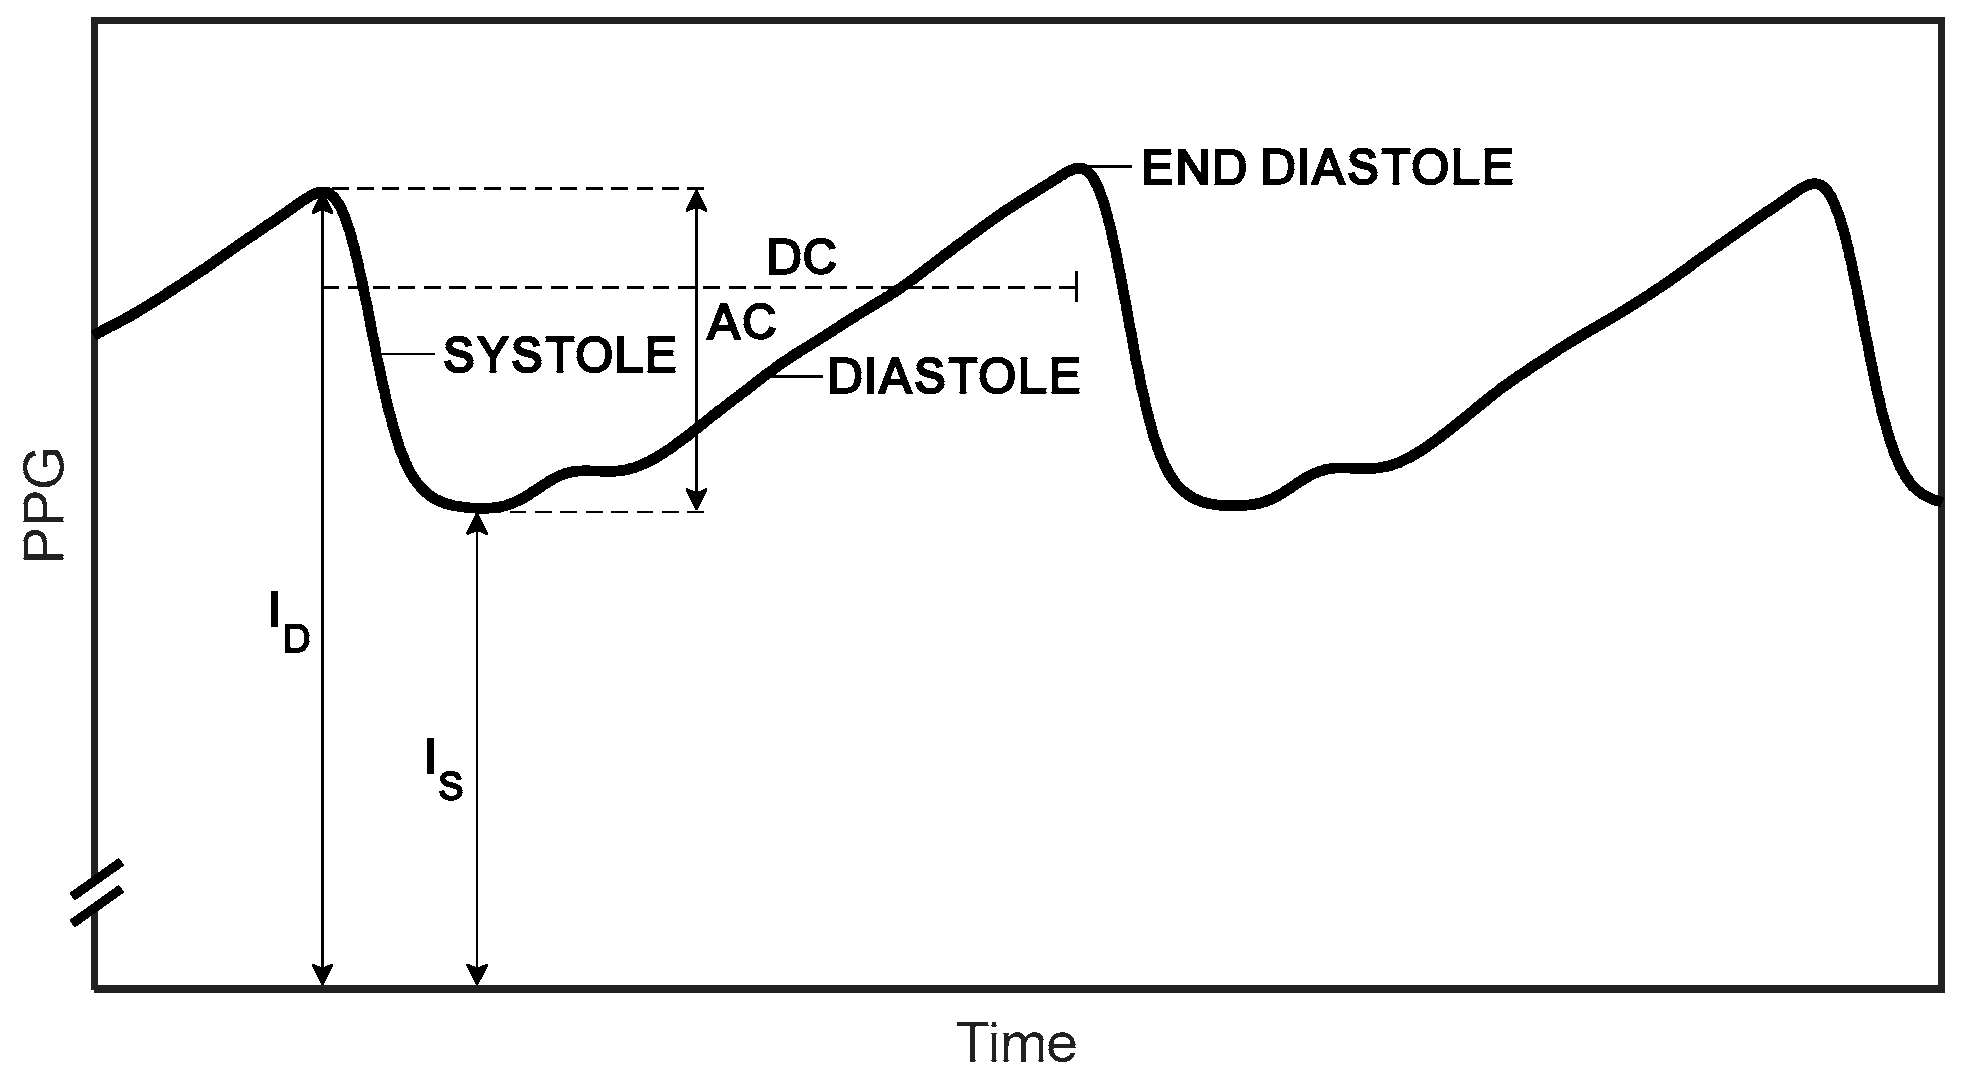
\includegraphics[width=1\textwidth]{Pictures/Graphs/PPG_pulse.png}
     \caption{Skematisk illustration af et PPG signal med AC og DC   komponent.}
     \label{fig:ppg_signal}
\end{figure}

\section{Beer-Bouguer-Lamberts lov}
Pulsoximetriske målinger bygger på Beer-Bouguer-Lamberts lov (herefter BBL), som beskriver attenuering af lys gennem et absorberende og homogent, ikke spredende, medie \cite{Tuchin2015,Pedrotti2017}. Loven kan formuleres på to ækvivalente måder.

\subsection{Intensitetsformulering}

Intensitetsformuleringen af BBL, udtrykker den transmitterede intensitet som funktion af den indkommende intensitet, absorptionskoefficienten og materialets tykkelse:
\begin{equation}
    I = I_0 \cdot e^{-\mu_a  d}
    \label{eq:bbl_fysik}
\end{equation}
Hvor: \\ 
$I$ er den transmitterede lysintensitet  \\
$I_0$ er den indkommende lysintensitet \\
$\mu_a$ er den lineære absorptionskoefficient i $\si{cm^{-1}}$ \\
$d$ er tykkelsen af materialet i $\si{cm}$.

\subsection{Absorbansformulering}
\label{subsec:absorbans}

Indenfor kemi udtrykkes BBL ofte gennem absorbansen $A$, 
defineret som \cite{Webster1997}
\begin{equation}
    A(\lambda) = -\log_{10}\!\left(\frac{I(\lambda)}{I_0(\lambda)}\right).
    \label{eq:absorbans_def}
\end{equation}
Bemærk at ligning \ref{eq:absorbans_def} er en generel definition af
absorbans uafhængig af om BBL gælder. Når BBL er gyldig, kan 
absorbansen udtrykkes som
\begin{equation}
    A(\lambda) = \varepsilon(\lambda) \cdot C \cdot d,
    \label{eq:bbl_absorbans}
\end{equation}
hvor: \\
$\varepsilon(\lambda)$ er den molare absorptionskoefficient, også kaldet extinktionskoefficient og er en materialegenskab der beskriver hvor stærkt et mol af et stof absorberer lys ved en given bølgelængde, angives i enheden $\si{cm^{-1}.M^{-1}}$ \\
$C$ er molarkoncentrationen i $\si{M}$ \\
$d$ er tykkelsen af mediet i $\si{cm}$.

Sammenhængen mellem absorptionskoefficienten i ligning \ref{eq:bbl_fysik} og den molare absorptionskoefficient er
\begin{equation}
    \mu_a(\lambda) = \varepsilon(\lambda) \cdot C \cdot \ln(10).
    \label{eq:mu_epsilon}
\end{equation}
Forudsat at BBL er gyldig, er ligning \ref{eq:bbl_fysik} og ligning \ref{eq:bbl_absorbans} således ækvivalente formuleringer af den samme fysik. I denne rapport anvendes primært ligning \ref{eq:bbl_fysik}.

For et medium med flere uafhængige absorbere er absorbansen en sum af de individuelle bidrag:
\begin{equation}
    A(\lambda) = \sum_i \varepsilon_i(\lambda) \cdot C_i \cdot d.
    \label{eq:bbl_multi}
\end{equation}
Dette superpositionsprincip følger af at hver foton interagerer uafhængigt med de enkelte molekyler i væv.

BBL antager at attenuation udelukkende skyldes absorption, og at lys propagerer i en lige linje gennem vævet uden at sprede sig, altså at den optiske vejlængde er lig med den geometriske afstand $d$. 

I væv er denne antagelse ikke opfyldt, da spredning bidrager væsentligt til attenuationen \cite{Tuchin2015}. Det vil altså sige, at ligning \ref{eq:bbl_fysik} kun gælder når $\mu_a \gg \mu_s$, det vil sige, når man kun har med mere absorberende end spredende medier at gøre. Konsekvenserne af spredning behandles i afsnit \ref{subsec:spredning}, og en modificeret formulering af BBL præsenteres i afsnit \ref{sec:mbbl}.
\section{Optiske egenskaber af biologisk væv}
\label{sec:optik_vaev}

\subsection{Attenuation}
Attenuation beskriver tabet af lysintensitet gennem et medie. Den kan forklares af to mekanismer: absorption, hvor fotoner destrueres ved energioverdragelse til molekyler, og spredning, hvor fotoner omdirigeres fra deres oprindelige udbredelsesretning. 

Den totale attenuationskoefficient er:
\begin{equation}
    \mu_t = \mu_a + \mu_s
    \label{eq:mu_total}
\end{equation}
hvor $\mu_a$ og $\mu_s$ er henholdsvis absorptions- og 
spredningskoefficienterne i $\si{cm^{-1}}$.

Et grundlæggende problem for pulsoximetri er, at det ud fra den målte intensitet alene ikke kan afgøres, om tabet skyldes ændret absorption eller ændret spredning. For at modellere væv korrekt må begge mekanismer karakteriseres.

\subsection{Absorption i væv}
Absorptionskoefficienten afhænger af bølgelængden og af 
koncentrationen af de absorberende molekyler i vævet, primært 
$\text{HbO}_2$, $\text{Hb}$, vand og melanin \cite{Jacques2013}.

I vinduet mellem ca. \SI{600}{nm} og \SI{1000}{nm} 
er absorptionen fra vand, melanin og øvrige vævskomponenter 
relativt lav, samtidig med at absorptionskoefficienterne for 
$\text{HbO}_2$ og $\text{Hb}$ er tilstrækkeligt forskellige til 
at muliggøre diskrimination, dette ses i figur \ref{fig:coeff_vs_wavelength}.
Ved kortere bølgelængder (under \SI{600}{nm}) dominerer 
absorption fra hæmoglobin og melanin, hvilket begrænser 
penetrationsdybden, mens absorption fra vand dominerer ved 
bølgelængder over \SI{1000}{nm} \cite[Fig.~(10.3)]{Tuchin2015}.

Ved overgangen mellem luft og væv opstår der desuden Fresnel-refleksion, fordi brydningsindekset ændrer sig ved grænsefladen \cite[s.~3]{Tuchin2015}. Dette bidrager til det samlede optiske tab og er en del af grunden til, at den målte transmission afhænger af både væv og målegeometri.

\begin{figure}[htbp]
    \centering
    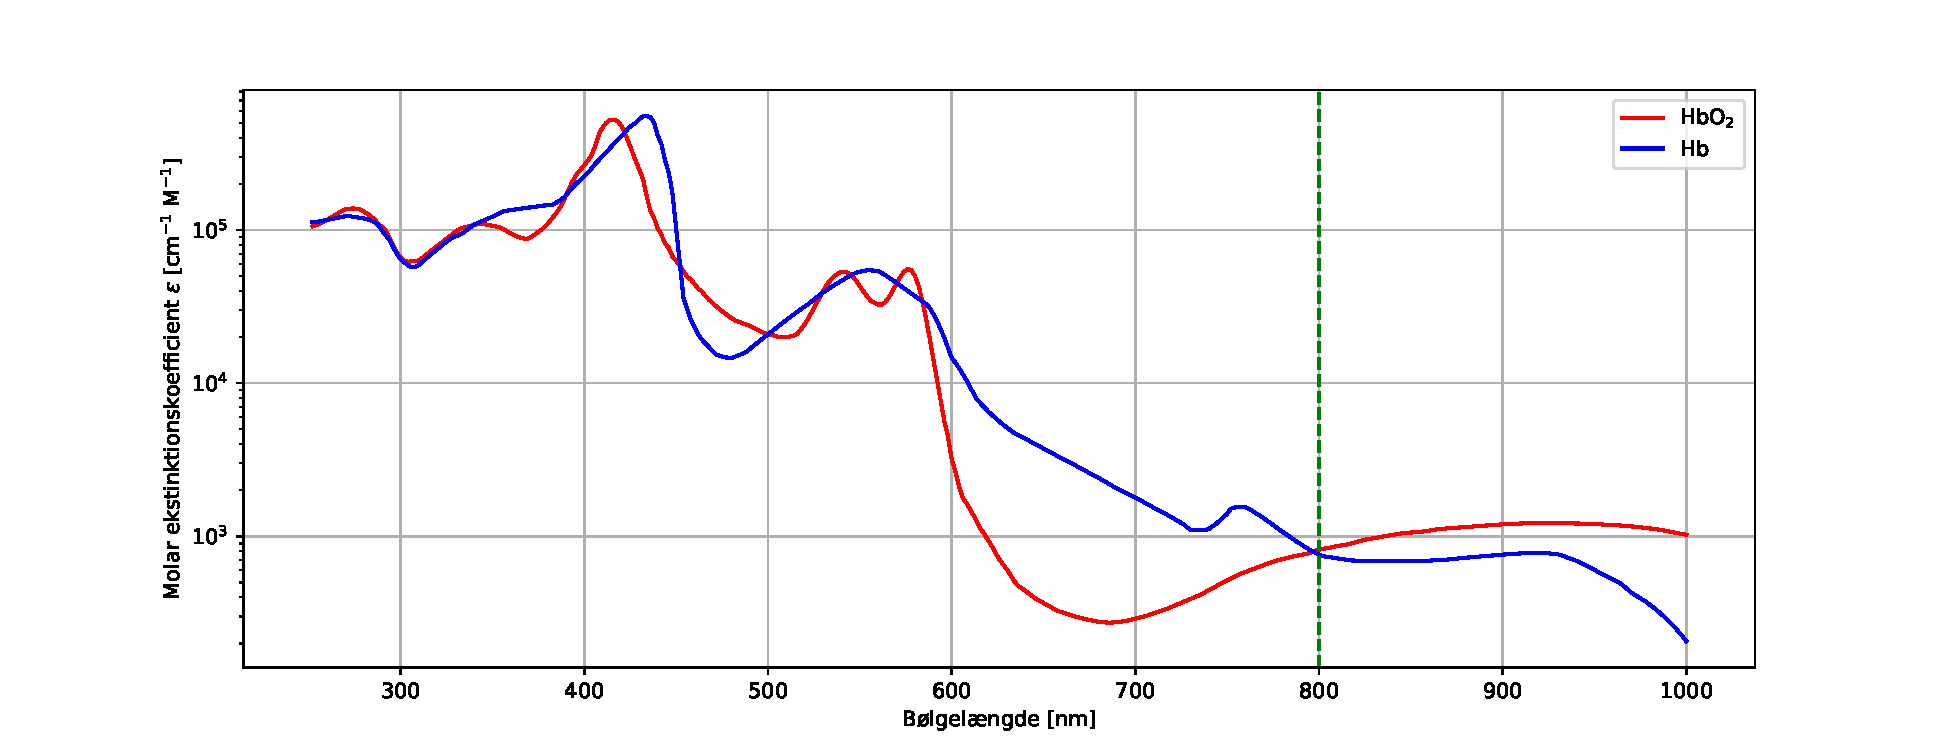
\includegraphics[width=1\textwidth]{Pictures/Graphs/extinction_spectra.pdf}
    \caption{Molare absorptionskoefficienter for $\text{HbO}_2$ 
    og $\text{Hb}$ som funktion af bølgelængden. En af flere 
    isosbestiske punkter er markeret ved \SI{800}{nm}. 
    \parencite{Prahl1998}}
    \label{fig:coeff_vs_wavelength}
\end{figure}

Ved et isosbestisk punkt (eksempelvis ca.\ \SI{800}{nm}) er absorptionskoefficienterne for $\text{HbO}_2$ og $\text{Hb}$ identiske: $\varepsilon_{\text{HbO}_2}(\SI{800}{nm}) = \varepsilon_{\text{Hb}}(\SI{800}{nm})$ \cite{Prahl1998}. En måling her er derfor uafhængig af iltmætningen i den simple Hb/HbO$_2$-model og kan i dette projekt betragtes som en mulig reference, selvom den ikke kan bruges til at skelne mellem $\text{HbO}_2$ og $\text{Hb}$.

\subsection{Spredning i væv}
\label{subsec:spredning}
Spredning i biologisk væv stammer fra strukturer over et bredt størrelsesinterval: fra molekylær skala op til celleorganeller, røde blodlegemer og kollagenfibre. Det afgørende parameter er forholdet mellem partikelstørrelse og bølgelængde.

\paragraph{Rayleigh-spredning} dominerer når partiklerne er væsentligt mindre end bølgelængden. Hæmoglobinmolekylet har en diameter på ca.\ \SI{5}{nm} \cite{Erickson2009}, 100 til 200 gange mindre end de klassisk anvendte bølgelængder (\SI{660}{nm} og \SI{940}{nm}) \cite{Webster1997}, og kan derfor beskrives ved Rayleigh-tilnærmelsen. Spredningens intensitet er proportional med $\lambda^{-4}$ \cite{Pedrotti2017}:
\begin{equation}
    I_{\text{Rayleigh}} \propto \frac{1}{\lambda^4}
    \label{eq:rayleigh_prop}
\end{equation}
Forholdet mellem Rayleigh-spredning ved de to klassiske 
bølgelængder bliver:
\begin{equation}
    \frac{I_{660}}{I_{940}} = 
    \left(\frac{940}{660}\right)^4 \approx 4.11
    \label{eq:rayleigh_ratio}
\end{equation}
Rødt lys ved \SI{660}{nm} spredes altså ca.\ fire gange mere 
end NIR-lys ved \SI{940}{nm} fra rene Rayleigh-spredere. Dette forhold er et idealiseret eksempel og beskriver ikke den samlede vævsspredning, som i praksis domineres af større of forskellige spredere.

\paragraph{Mie-spredning} dominerer når partikelstørrelsen er sammenlignelig med eller større end bølgelængden, dette er relevant for celleorganeller, røde blodlegemer ($\sim$\SI{7}{\micro\meter}) og kollagenfibre \cite{DiezSilva2010} \cite[s.~4-6]{Tuchin2015}. Mie-spredning har en svagere bølgelængdeafhængighed end Rayleigh og er desuden overvejende fremadrettet, i modsætning til den tilnærmelsesvist isotropisk ($g=0$) Rayleigh-spredning \cite[s. 13]{Tuchin2015}.

\paragraph{Anisotropi.} Da de dominerende spredere i biologisk væv (celleorganeller, røde blodlegemer og kollagenfibre) alle falder i Mie-regimet, er vævsspredning som helhed ikke isotrop. Anisotropien kvantificeres med faktoren \cite[s.~13]{Tuchin2015}:
\begin{equation}
    g = \langle \cos \theta \rangle
    \label{eq:anisotropy}
\end{equation}
hvor $\langle \cdot \rangle$ betegner gennemsnittet over 
alle spredningshændelser, og $\theta$ er spredningsvinklen 
i forhold til indfaldsretningen. Værdien $g = 0$ svarer til isotropisk spredning, $g = 1$ til fuld fremadspredning og $g = -1$ til fuld tilbagespredning \cite[s.~13]{Tuchin2015}. Dette kan visualiseres i figur \ref{fig:anisotropi}:

\begin{figure}[htbp]
    \centering
    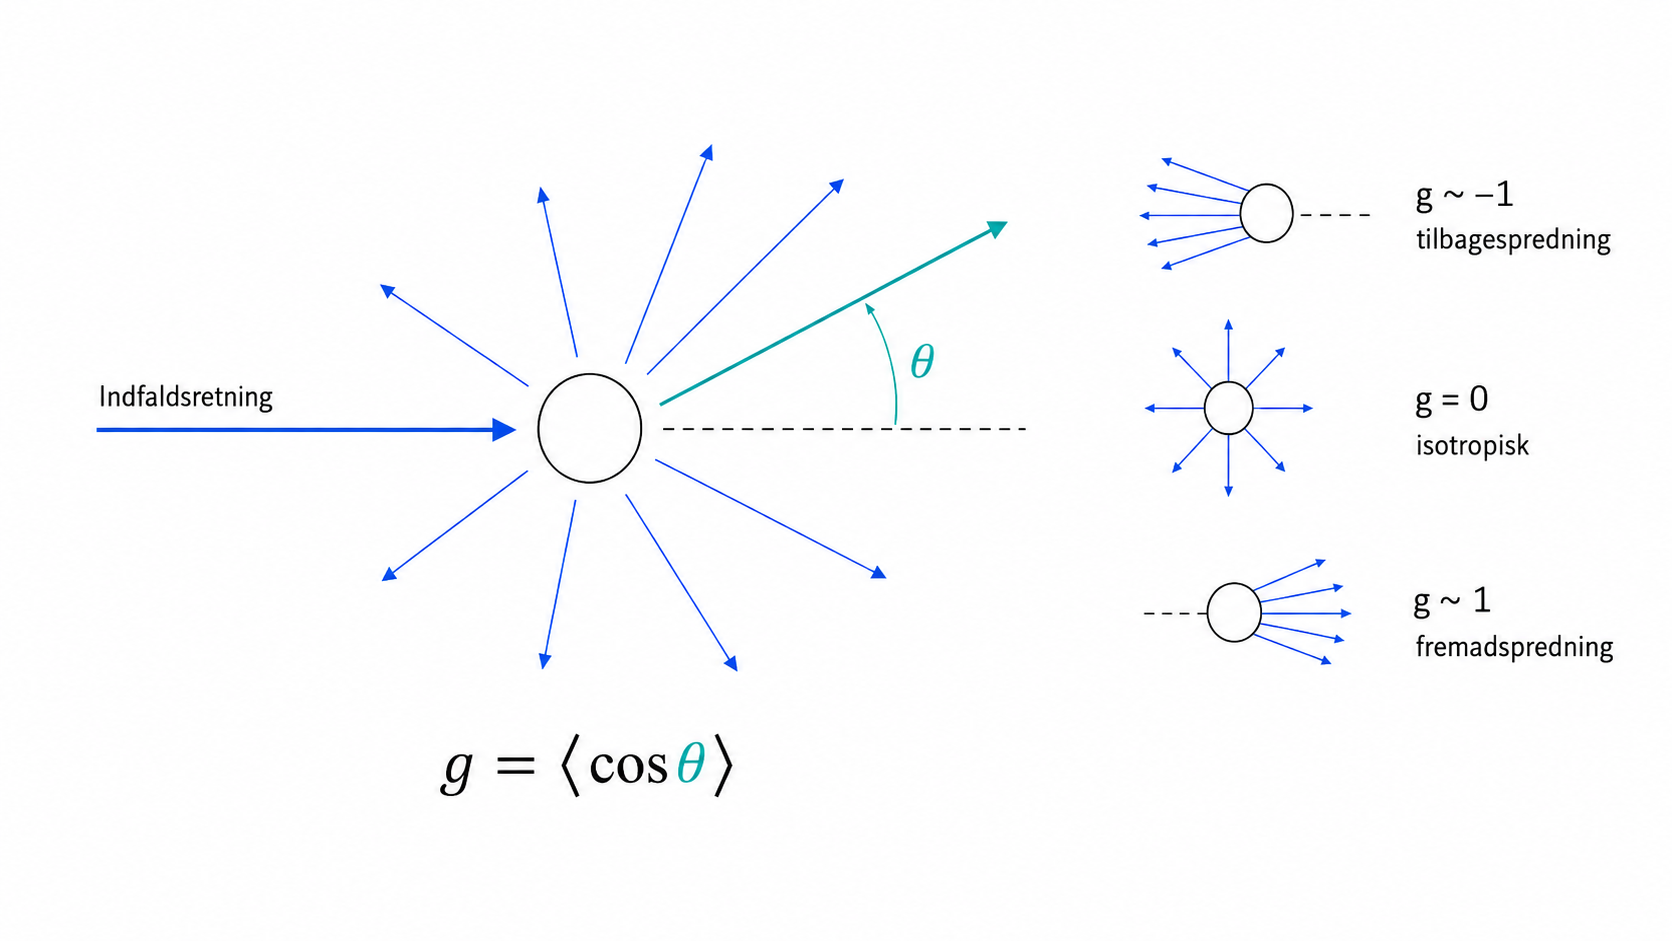
\includegraphics[width=1\textwidth]{Pictures/Graphs/Anisotropi.png}
    \caption{LLM-assisteret illustration af anisotropisk spredning i biologisk væv. Anisotropifaktoren $g = \langle \cos \theta \rangle$ beskriver den gennemsnitlige spredningsretning, hvor $g = 0$ svarer til isotropisk spredning, mens $g \sim 1$ og $g \sim -1$ svarer til henholdsvis fremad- og tilbagespredning. For biologisk væv er $g \approx 0.7$ til $0.95$.}
    \label{fig:anisotropi}
\end{figure}

\paragraph{Reduceret spredningskoefficient.} Da $\mu_s$ ikke alene beskriver effekten af fremadrettet anisotrop spredning, indføres den reducerede spredningskoefficient \cite[Eq.~(1.21)]{Tuchin2015}:
\begin{equation}
    \mu_s' = \mu_s (1 - g)
    \label{eq:mu_s_red}
\end{equation}
$\mu_s'$ kan tolkes som den ækvivalente isotrope 
spredningskoefficient, der ville give samme effektive 
foton-diffusion som den faktiske anisotrope spredning.

\paragraph{Bølgelængdeafhængighed.} Empirisk, følger den 
reducerede spredningskoefficient en såkaldt power-law-relation 
\cite{Jacques2013}:
\begin{equation}
    \mu_s'(\lambda) \propto \lambda^{-b}
    \label{eq:mu_scatter_wavelength}
\end{equation}
Eksponenten $b$ afspejler den relative andel af Rayleigh- og 
Mie-spredere i vævet. Ren Rayleigh-spredning ville give $b = 4$, 
ren Mie-spredning $b \approx 0$. For hudvæv ligger $b$ typisk 
mellem 0.7 og 1.5, afhængigt af alder, målemetode og hudtype 
\cite{Jacques2013}, hvilket afspejler at hud indeholder en 
blanding af spredere fra begge regimer.

\section{Modificeret Beer-Lamberts lov}
\label{sec:mbbl}

Da BBL ikke tager højde for spredning, er den utilstrækkelig til beskrivelse af lystransmission gennem biologisk væv. Den modificerede Beer Lamberts lov (MBBL) inkluderer et spredningsled \cite[Eq.~(10.6)]{Tuchin2015} \cite[Eq.~(2)]{Barstow2019}:
\begin{equation}
    I_t = I_0 e^{-G - \varepsilon C l}
    \label{eq:mbbl}
\end{equation}
eller ækvivalent:
\begin{equation}
    \ln\!\left(\frac{I_0}{I_t}\right) = G + \varepsilon C l
    \label{eq:mbbl_ln}
\end{equation}
Hvor: \\ 
$l$ er den effektive optiske vejlængde\\ 
$G$ er et dimensionsløst led, der samler bidrag fra spredning og målegeometri\\
$\varepsilon C l$ er bidraget fra absorption.

Ved transmissionsmåling kan $G$ fortolkes som et samlet tabsled forbundet med fotoner, der som følge af spredning og geometri ikke når detektoren. $G$ er et geometrisk tab der afhænger af spredningsgeometrien og måleopsætningen, og er ikke en simpel funktion af anisotropifaktoren $g$ alene.

Da fotoner spredes undervejs, er den effektive optiske vejlængde $l$ længere end den geometriske afstand $d$. Forholdet beskrives af den differentielle vejlængdefaktor (DPF):
\begin{equation}
    \text{DPF} = \frac{l}{d}
    \label{eq:dpf}
\end{equation}
For typisk fingervæv ligger $\text{DPF} \approx 4$ til $7$ \cite{Jacques2013} \cite{Barstow2019}, hvilket vil sige at fotonerne i gennemsnit rejser 4–7 gange længere end den lige linje fra LED til detektor. Litteraturen rapporterer DPF-værdier i denne størrelsesorden, men DPF afhænger af vævstype, bølgelængde og målegeometri. 

Da $l = \text{DPF} \cdot d$ indgår direkte i absorptionsleddet $\varepsilon C l$ i ligning \ref{eq:mbbl_ln}, skalerer DPF absorptionsleddet $\varepsilon Cl$ proportionalt. En større effektiv vejlængde betyder at fotonerne møder mere hæmoglobin, og dermed vil den geometriske afstand $d$ undervurdere den faktiske optiske vejlængde og dermed ikke beskrive den målte attenuation korrekt. Da spredning er bølgelængdeafhængig, er DPF ikke identisk ved \SI{660}{nm} og \SI{940}{nm}, hvilket har konsekvenser for ratio-of-ratios-modellen, dette behandles i afsnit \ref{sec:ratio_of_ratios}.

\subsection{Gennemsnitlig absorptionskoefficient}
Den gennemsnitlige absorptionskoefficient i blodet afhænger af iltmætningen:
\begin{equation}
    \varepsilon(\lambda) = \varepsilon_{\text{HbO}_2}(\lambda) \cdot S + \varepsilon_{\text{Hb}}(\lambda) \cdot (1 - S)
    \label{eq:epsilon_mix}
\end{equation}
Hvor: \\ 
$\varepsilon_{\text{HbO}_2}$ og $\varepsilon_{\text{Hb}}$ adskiller sig som følge af O$_2$-bindingen til hæmgruppen, ses i figur \ref{fig:coeff_vs_wavelength}.
$S$ repræsenterer oxyhæmoglobinfraktionen.

Indsættes ligning \ref{eq:epsilon_mix} i ligning \ref{eq:mbbl_ln}, fås:
\begin{equation}
    \ln\!\left(\frac{I_0}{I_t}\right) = G + \varepsilon_{\text{Hb}} C l + C l (\varepsilon_{\text{HbO}_2}- \varepsilon_{\text{Hb}}) \cdot \text{S}
    \label{eq:mbbl_so2}
\end{equation}
For at isolere $\text{S}$ fra ligning \ref{eq:mbbl_so2} skal parametrene $G$, $C$ og $l$ kendes. Disse parametre varierer imidlertid betydeligt fra person til person, hvilket gør direkte beregning upraktisk. Pulsoximetri reducerer afhængigheden af ukendte, absolutte baggrundsbidrag ved at udnytte den pulsatile ændring i arterielt blodvolumen.

\section{Målekonfigurationer}
\label{sec:målekonfigurationer}

\begin{figure}[htbp]
    \centering
    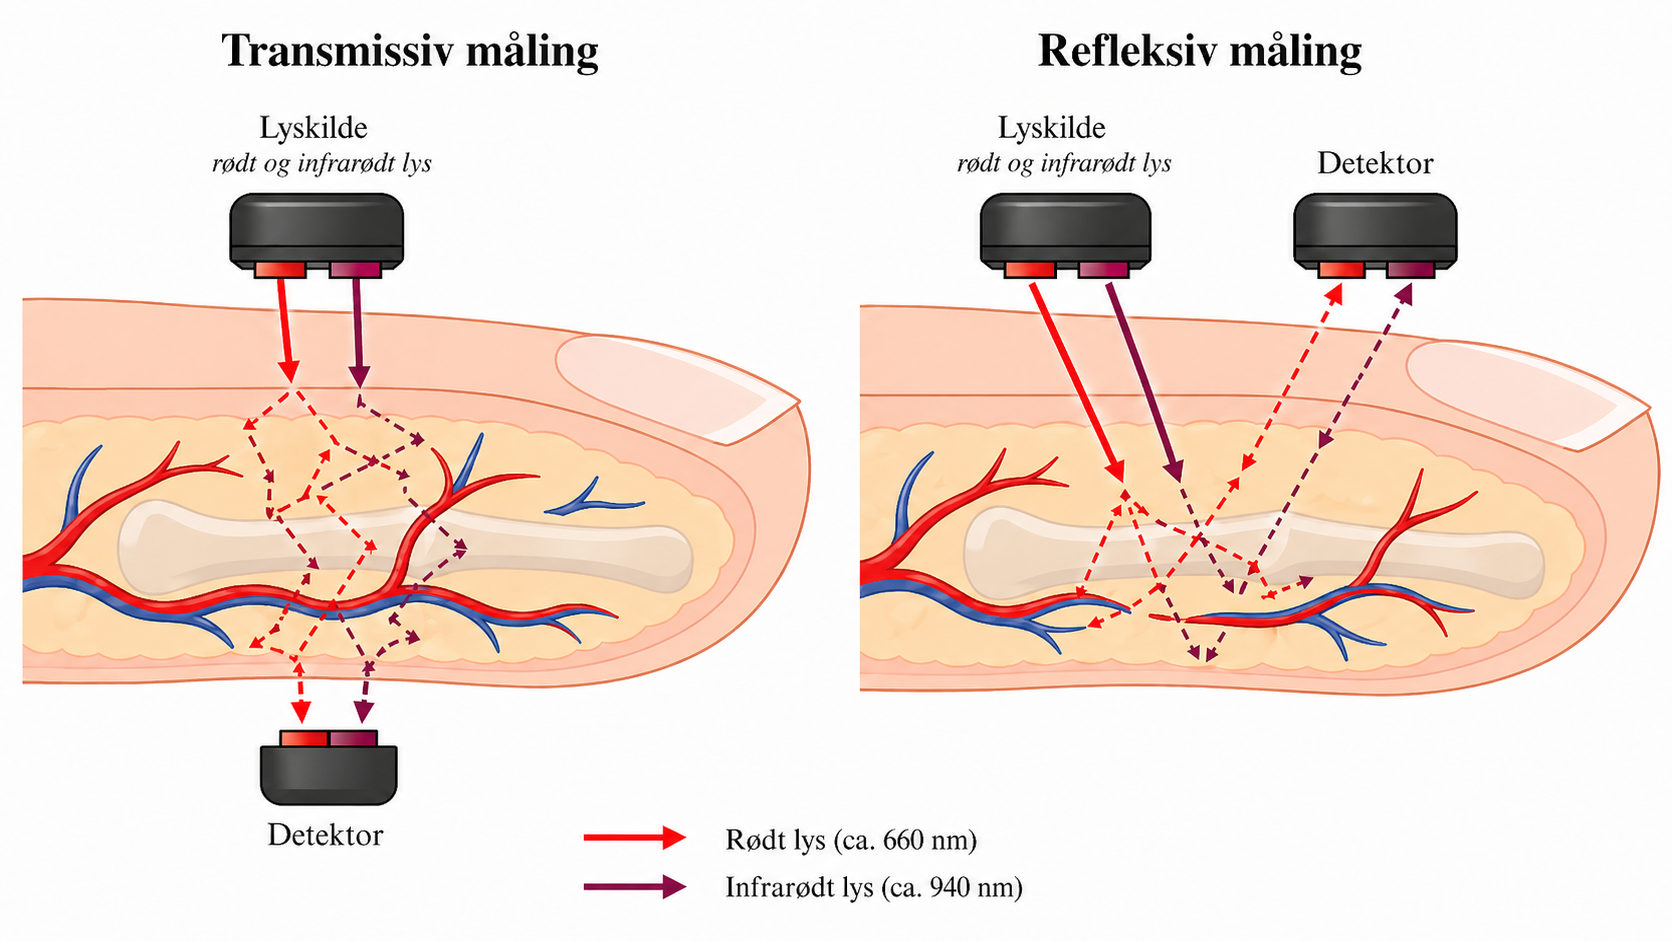
\includegraphics[width=1\textwidth]{Pictures/Other/measurement_methods.png}
    \caption{LLM-assisteret illustration af princippet for transmissionsmåling (venstre) og refleksionsmåling (højre) i pulsoximetri. Figuren er baseret på principperne beskrevet i \cite[S.~87--88]{Webster1997}.}
    \label{fig:målekonfigurationer}
\end{figure}

Pulsoximetri kan udføres i to optiske konfigurationer (figur \ref{fig:målekonfigurationer}). Ved transmissionsmåling placeres lyskilde og detektor på modsatte sider af vævet, typisk fingerspids, øreflip eller hos spædbørn, fod eller tå. Lyset gennemtrænger vævet, og detektoren registrerer den transmitterede intensitet \cite[S.~87--88]{Webster1997}.

Ved refleksionsmåling placeres lyskilde og detektor på samme side, og detektoren registrerer det tilbagespredte lys. Pulsoximeteret placeres normalt på brystet, panden eller håndleddet, hvilket gør konfigurationen mere fleksibel og velegnet til flere  placeringer på kroppen \cite[S.~87--88]{Webster1997}.

\section{Pulsoximetrisk måleprincip}
\label{sec:pulseox_princip}

\subsection{Reduktion af ukendte parametre}
Ved at betragte forholdet mellem intensiteterne ved systole og diastole kan afhængigheden af flere ukendte parametre reduceres. Intensiteterne udtrykkes via ligning \ref{eq:mbbl} \cite[s.126--129]{Webster1997}. Her anvendes $\varepsilon = \varepsilon(\lambda, S)$ som defineret i ligning \ref{eq:epsilon_mix}. $S$ antages konstant mellem systole og diastole, det er blodvolumen, ikke iltmætningen, der varierer med pulsen:
\begin{equation}
    I_D = I_0 e^{-G_D - \varepsilon C_D l_D}
    \label{eq:i_diastole}
\end{equation}
\begin{equation}
    I_S = I_0 e^{-G_S - \varepsilon C_S l_S}
    \label{eq:i_systole}
\end{equation}
Forholdet mellem de to giver:
\begin{equation}
    \frac{I_S}{I_D} = \exp\!\Big[(G_D - G_S) + \varepsilon(C_D l_D - C_S l_S)\Big]
    \label{eq:is_id_ratio}
\end{equation}
Under antagelse af at spredningsgeometrien ikke ændrer sig væsentligt mellem systole og diastole ($G_D \approx G_S$), reducerer dette til:
\begin{equation}
    \ln\!\left(\frac{I_S}{I_D}\right) \approx \varepsilon(C_D l_D - C_S l_S)
    \label{eq:ln_ratio_simplified}
\end{equation}
Hermed er den ukendte parameter $G$ elimineret, så det resterende led kan fortolkes som den pulsatile ændring i den absorberende del af den optiske vej.

\subsection{Ratio of ratios}
\label{sec:ratio_of_ratios}
Ligning \ref{eq:ln_ratio_simplified} skrives for begge bølgelængder (\SI{660}{nm} og \SI{940}{nm}), og forholdet mellem dem defineres som:
\begin{equation}
    R = \frac{\ln(I_S / I_D)_{\SI{660}{nm}}}{\ln(I_S / I_D)_{\SI{940}{nm}}} 
    \approx \frac{(AC/DC)_{\SI{660}{nm}}}{(AC/DC)_{\SI{940}{nm}}}
    \label{eq:ratio_of_ratios}
\end{equation}
Tilnærmelsen $\ln(I_S/I_D) \approx AC/DC$ gælder da AC komponentens amplitude er lille i forhold til DC niveauet. I en idealiseret model er $R$ primært bestemt af de relative absorptionsforskelle mellem de to bølgelængder. I praksis påvirkes $R$ også af bølgelængdeafhængig spredning, forskellige effektive optiske vejlængder og sensorens geometri.

\subsection{Empirisk kalibrering}
Teoretisk kan $\text{SpO}_2$ udledes analytisk fra $R$ ved hjælp af kendte absorptionskoefficienter. I praksis er de forenklende antagelser (bl.a.\ $G_D \approx G_S$, samt neglekt af spredningens bølgelængdeafhængighed) ikke fuldstændigt opfyldt. Derfor kalibreres forholdet mellem $R$ og $\text{SpO}_2$ empirisk ved at sammenligne pulsoximetriske målinger med samtidige blodgasanalyser ($\text{SaO}_2$) på frivillige forsøgspersoner. Den resulterende kalibreringskurve kan i en simpel model tilnærmes med et lineært udtryk \cite{Webster1997}:
\begin{equation}
    \text{SpO}_2 = a - b \cdot R
    \label{eq:spo2_calibration}
\end{equation}
hvor $a$ og $b$ er empirisk bestemte konstanter, som f.eks. kan kalibreres ud fra eksisterende pulsoximetre. Som tommelfingerregel rapporteres ofte at $\text{SpO}_2 \approx 100\,\%$ ved $R = 0.4$, mens $\text{SpO}_2 \approx 85\,\%$  ved $R = 1$ \cite{Webster1997}.

\subsection{Tidsmultipleksing}

Tidsmultipleksing er en teknik til at dele en enkelt målekanal mellem flere signalkilder ved at tildele hver kilde et bestemt tidsinterval, hvor kun den pågældende kilde er aktiv. Opsætningen af det analoge pulsoximeter bygger på princippet om tidsmultipleksing, og tillader brug af de to LED'er med det præcist samme kredsløb, uden at blande signalerne sammen \cite[s.~126--129]{Webster1997}.

Hvis både \SI{940}{nm} og \SI{660}{nm} LED'erne var tændt på samme tid, ville det ikke være muligt for fotodioden at adskille det røde eller infrarøde signal, da fluxbidraget på det fotosensitive areal ville være en sum af de to LED'ernes signaler. Derfor, kender man ikke forskellen mellem de to signaler, kan man ikke beregne $R$ i ratio of ratios, og dermed ikke finde en tilstrækkelig tilnærmelse af $\text{SpO}_2$.

Ud over LED-målingerne inkluderes en tredje måling, hvor begge LED'er er slukkede. Denne "mørkemåling" registrerer bidrag der altså ikke stammer fra de to LED'er som f.eks. fotodiodens mørkestrøm, DC offset, \SI{50}{Hz} støj og andre støjkilder. Ved at trække mørkemålingen fra de to LED-målinger isoleres den lysafhængige komponent fra hver bølgelængde.

Målingerne køres i cyklus i rækkefølgen: \SI{940}{nm}, \SI{660}{nm}, mørkemåling. Tabel \ref{tab:maalinger} viser en komplet målecyklus.

\begin{table}[h]
\centering
\caption{Oversigt over en komplet målecyklus}
\label{tab:maalinger}
\begin{tabular}{lll}
\toprule
Måling & 940 nm LED& 660 nm LED\\
\midrule
Måling 1 & Tændt & Slukket \\
Måling 2 & Slukket & Tændt \\
Måling 3 & Slukket & Slukket \\
\bottomrule
\end{tabular}
\end{table}


\section{Halvlederfysik}
\label{sec:halvleder}

Fremstillingen i dette og efterfølgende afsnit om optoelektroniske komponenter (afsnit \ref{sec:optoelektroniske_komponenter}) bygger primært på \cite[Kap.~16--18]{Saleh2007}, medmindre andet er angivet.

Konduktivitet er en egenskab der beskriver et materiales evne til at lede elektricitet. En halvleder er et krystallinsk materiale med en elektrisk konduktivitet mellem en leder og en isolator. 
Konduktiviteten kan ændres ved at variere temperaturen, doping eller belysning. Elektronik bruger typisk halvledere lavet af silicium (Si), mens optoelektronik ofte benytter legeringer af flere grundstoffer. Legeringer med to, tre eller fire grundstoffer kaldes henholdsvis binære, ternære og kvaternære halvledere.

Behovet for legeringer stammer fra ønsket om at skræddersy materialets egenskaber, herunder:
\begin{itemize}
    \item et specifikt båndgab (og dermed en specifik bølgelængde)
    \item temperaturstabilitet
    \item billigere eller nemmere fabrikation
    \item høj lysstyrke ved emission
    \item lav defektrate i krystalgitteret
\end{itemize}

\subsection{Båndteori}

Forskellen mellem halvledere, isolatorer og metaller illustreres i figur \ref{fig:de tre bånd}. Hver klasse repræsenteres med to bånd: et valensbånd og et ledningsbånd. 

\begin{figure}[htbp]
    \centering
    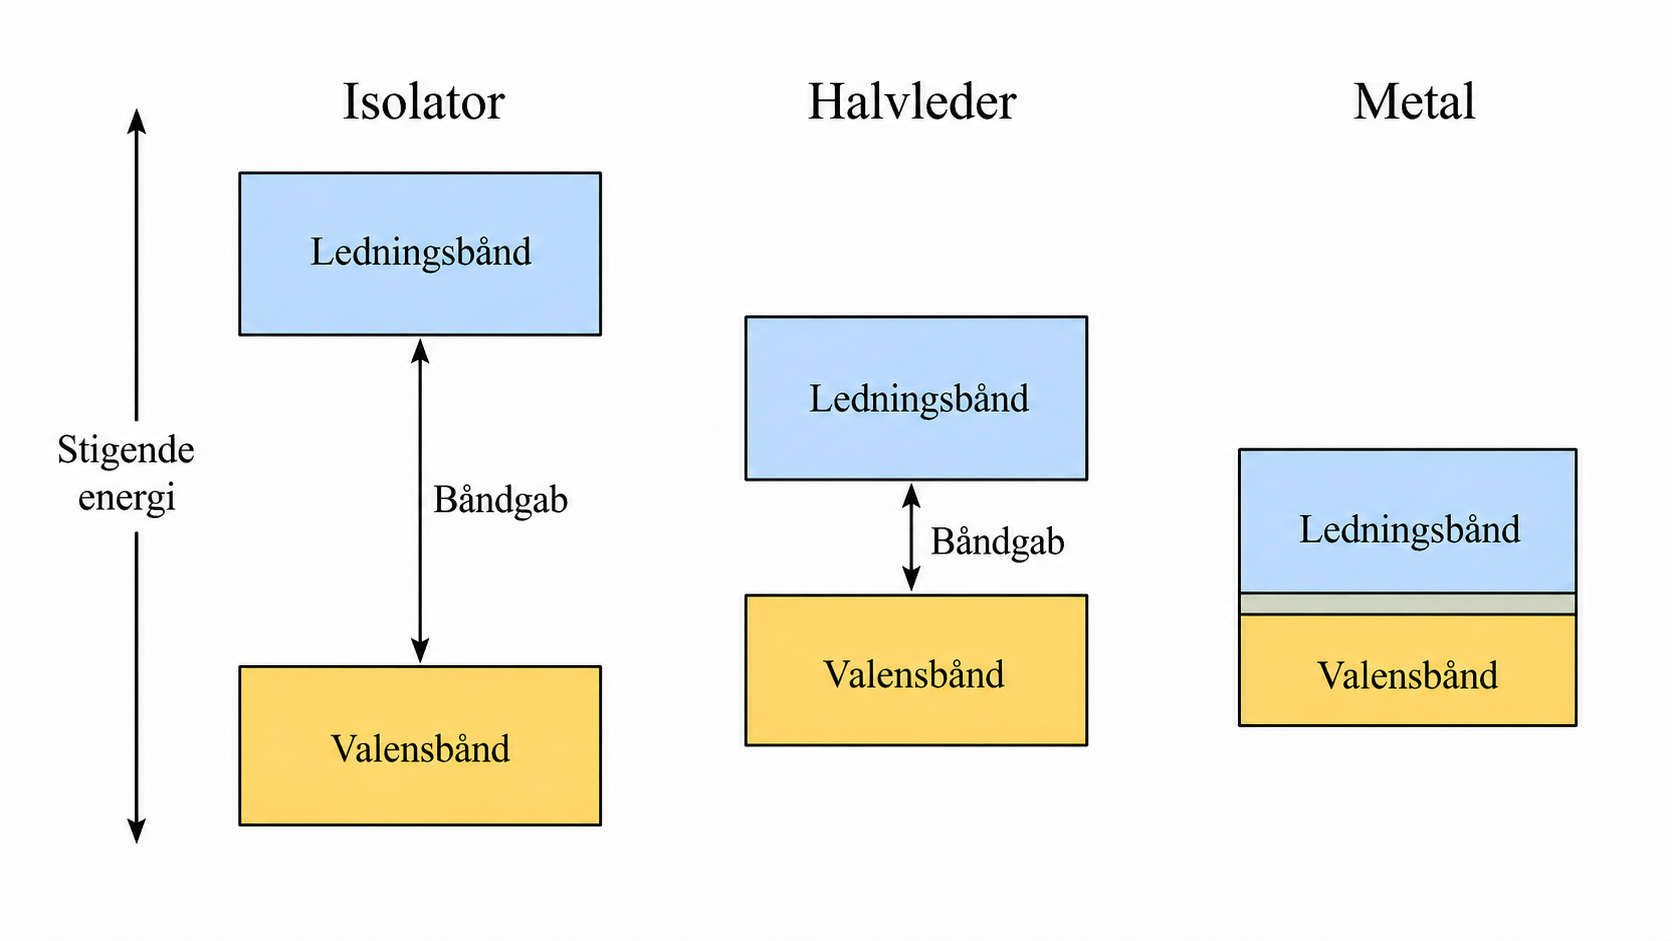
\includegraphics[width=1\textwidth]{Pictures/Other/båndgab_faststof.png}
    \caption{LLM-assisteret skematisk illustration af båndstrukturen for de tre faststoftyper.
    De gule bokse repræsenterer valensbåndet og de blå ledningsbåndet.}
    \label{fig:de tre bånd}
\end{figure}

Valensbåndet består af de energiniveauer hvor materialets valenselektroner befinder sig i grundtilstanden. I silicium, der har fire valenselektroner per atom, er valensbåndet helt fyldt ved $T = \SI{0}{K}$. Elektroner i et fyldt valensbånd kan ikke bidrage til en elektrisk strøm, da der ikke er ledige energi-niveauer at flytte sig til. Energien der kræves for at løfte en elektron fra valensbåndet til ledningsbåndet, hvor den frit kan bevæge sig, kaldes båndgabsenergien $E_g$ og angives typisk i enheden elektronvolt og relateres til Joules som:
\begin{equation}
    1 \ \text{eV} = \SI{1.602e-19}{J}.
\end{equation}

Ved $T > \SI{0}{K}$ vil termisk energi excitere nogle elektroner til ledningsbåndet. Den exciterede elektron efterlader en tom plads i valensbåndet, betegnet et hul. Hullet kan beskrives som en positivt ladet kvasi-partikel der bevæger sig i valensbåndet, mens den exciterede elektron bevæger sig i ledningsbåndet. Begge ladningsbærere bidrager til konduktiviteten ved påførelse af et eksternt elektrisk felt, og konduktiviteten stiger derfor med temperaturen, da flere elektron-hul par dannes.

Forskellen mellem metaller, halvledere og isolatorer ligger i størrelsen af deres båndgab. I metaller er et bånd delvist fyldt eller også overlapper valens- og ledningsbånd, så ladningsbærere kan bevæge sig uden termisk excitation over et båndgab. I isolatorer er båndgabet så stort ($> \SI{4}{eV}$) at termisk excitation ved stuetemperatur ikke er nok til at excitere elektroner til ledningsbåndet. Halvledere ligger imellem, med båndgab i intervallet \SIrange{0.5}{3}{eV}, hvilket gør deres konduktivitet kontrollerbar via temperatur, doping og belysning.

\subsection{Båndgab og foton-energi}

Når en exciteret elektron rekombinerer med et hul, frigives båndgabsenergien $E_g$. I direkte båndgab-materialer (se næste afsnit) frigives denne energi som en foton. Sammenhængen mellem 
foton-energi og bølgelængde er:
\begin{equation}
\label{eq:bølgelængde_energi}
    E = \frac{hc}{\lambda},
\end{equation}
hvor $h = \SI{6.626e-34}{J\cdot s}$ er Plancks konstant og $c$ er lysets hastighed. Med $E$ angivet i eV og $\lambda$ i nm approksimeres udtrykket som:
\begin{equation}
    E[\text{eV}] \approx \frac{1240}{\lambda [\text{nm}]}
\end{equation}

Som eksempel: AlGaInP er en kvaternær halvleder med båndgabsenergi $E_g \approx \SI{1.9}{eV}$. Når elektroner exciteres over båndgabet og efterfølgende rekombinerer, emitteres fotoner med denne energi. Den tilsvarende bølgelængde er:
\begin{equation}
    \lambda = \frac{1240}{1.9} \approx 652.6\ \text{nm},
\end{equation}
svarende cirka til den røde LED anvendt i dette projekt. Tabel \ref{tab:faststoffer} viser båndgab og typiske anvendelser for relevante materialer.

\begin{table}[h]
\centering
\caption{Båndgabsenergier for udvalgte halvledermaterialer ved 
\SI{300}{K}, samt deres typiske anvendelse. Værdier fra 
\cite[Tabel~16.3-1]{Saleh2007}.}
\label{tab:faststoffer}
\begin{tabular}{@{}lSll@{}}
\toprule
Materiale & {$E_g$ [eV]} & Type & Typisk anvendelse \\
\midrule
Germanium (Ge)  & 0.67 & Indirekte & NIR-fotodiode \\
Silicium (Si)   & 1.12 & Indirekte & Fotodiode, anden elektronik \\
GaAs            & 1.42 & Direkte   & NIR LED, laser \\
AlGaInP         & 1.9  & Direkte   & Rød LED (\SI{660}{nm}) \\
GaN             & 3.4  & Direkte   & Blå/UV LED \\
\bottomrule
\end{tabular}
\end{table}

\subsection{Direkte og indirekte båndgab}
\label{subsec:direkte_indirekte}

Den simple båndmodel i figur \ref{fig:de tre bånd} kan udvides ved at inkludere ladningsbærernes momentum. I et $E$-$k$-diagram plottes elektronenergien $E$ som funktion af bølgevektoren $k$ eller ækvivalent af krystalmomentummet $\hbar k$. Figur \ref{fig:direct_indirect_bandgap} viser to repræsentative diagrammer.

Når en elektron exciteres til ledningsbåndet med en energi der overstiger $E_g$, vil den hurtigt afgive overskydende energi til gittervibrationer (fononer) og falde til ledningsbåndets minimum. Denne proces, kaldet termalisering, sker på pikosekund tidsskala og er væsentligt hurtigere end den efterfølgende rekombination, som typisk tager nano- til mikrosekunder. Tilsvarende termaliserer hullet til valensbåndets maksimum. Rekombination foregår derfor mellem disse to ekstrema.

\paragraph{Direkte båndgab.} I et materiale med direkte båndgab ligger ledningsbåndets minimum og valensbåndets maksimum ved samme $k$-værdi (figur \ref{fig:direkte_bandgap}). Rekombination kan ske ved emission af en enkelt foton med energi $E_g$, da fotonen bærer energi men forsvindende lille momentum. Foton-emission svarer dermed til en vertikal overgang i $E$-$k$-diagrammet, hvor elektronens $k$-værdi bevares. Denne proces er effektiv, og 
direkte halvledere som AlGaInP og GaAs anvendes derfor som 
lyskilder i LEDer og lasere.

\paragraph{Indirekte båndgab.} I et materiale med indirekte båndgab ligger ekstrema ved forskellige $k$-værdier (figur \ref{fig:indirekte_bandgap}). Rekombination kræver derfor samtidig deltagelse af en fonon for at bevare momentum, hvilket reducerer sandsynligheden for foton-emission betydeligt. Indirekte materialer som silicium er derfor ineffektive som lyskilder, men velegnede som fotodetektorer, fordi de kan absorbere fotoner med energi over båndgabet og generere ladningsbærere over et bredt spektralområde.

Denne distinktion forklarer komponentvalget i pulsoximetri: LEDerne er fremstillet af direkte halvledere (AlGaInP for \SI{660}{nm}, GaAs-baserede legeringer for \SI{940}{nm}), mens fotodioden er silicium-baseret.

\begin{figure}[htbp]
     \centering
     \begin{subfigure}[b]{0.48\textwidth}
         \centering
         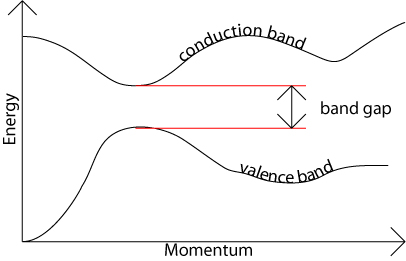
\includegraphics[width=\textwidth]{Pictures/Other/direct_bandgap.png}
         \caption{Direkte båndgab.}
         \label{fig:direkte_bandgap}
     \end{subfigure}
     \hfill
     \begin{subfigure}[b]{0.48\textwidth}
         \centering
         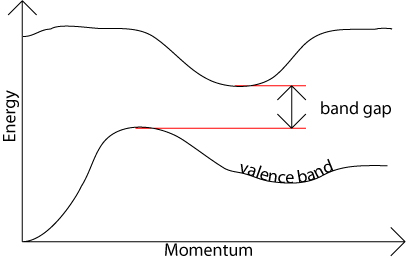
\includegraphics[width=\textwidth]{Pictures/Other/indirect_bandgap.png}
         \caption{Indirekte båndgab.}
         \label{fig:indirekte_bandgap}
     \end{subfigure}
     \caption{$E$-$k$-diagrammer for henholdsvis et materiale med 
     direkte (a) og indirekte (b) båndgab.}
     \label{fig:direct_indirect_bandgap}
\end{figure}

\subsection{Doping og pn-overgangen}

De elektriske og optiske egenskaber af en halvleder kan ændres markant ved kontrolleret introduktion af urenheder, kaldet doteringsstoffer. Doping ændrer koncentrationen af ladningsbærere i materialet og er fundamentet for stort set alle halvlederkomponenter.

Doteringsstoffer der bidrager med et overskud af valenselektroner kaldes donorer. For silicium (gruppe 14) anvendes typisk donorer fra gruppe 15, f.eks. fosfor eller arsen, der har en ekstra valenselektron sammenlignet med silicium. Den resulterende halvleder kaldes en n-type halvleder og har et overskud af frie elektroner.

Doteringsstoffer der mangler en valenselektron kaldes acceptorer. Typiske acceptorer for silicium kommer fra gruppe 13, f.eks. bor eller gallium. Den resulterende halvleder kaldes en p-type halvleder og har et overskud af huller.

Når en n-type og en p-type halvleder bringes i kontakt, dannes en pn-overgang, som er den fundamentale byggesten i både LEDer og fotodioder. Ved kontaktfladen diffunderer elektroner fra n-siden til p-siden og rekombinerer med huller, og omvendt. 

Resultatet er en zone uden frie ladningsbærere, kaldet depletionsregionen, hvor der opbygges et internt elektrisk felt der modvirker yderligere diffusion. I termisk ligevægt balancerer dette felt diffusionen, og der løber ingen netto-strøm gennem overgangen.

Pn-overgangens funktion afhænger af hvordan den biaseres:

\begin{description}
    \item[Forward bias.] Når der påføres en positiv spænding fra p-siden til n-siden, reduceres det interne felt, og ladningsbærere kan strømme over overgangen. Elektroner injiceres fra n-siden til p-siden og rekombinerer med huller. I direkte båndgab-materialer udsendes en foton ved hver rekombination, dette er princippet bag en LED.
    
    \item[Reverse bias.] Når den modsatte spænding påføres, forstørres depletionsregionen og det interne felt, og uden belysning flyder kun en lille mørkestrøm. Hvis der absorberes en foton i eller nær depletionsregionen, opstår et elektron-hul-par der separeres af det interne felt, hvilket resulterer i en lille fotostrøm. Dette er princippet bag en fotodiode.
\end{description}

\subsection{Rekombination og fotonemission}

Den modsatte proces til elektron-hul-generation er rekombination, hvorpå en elektron i ledningsbåndet henfalder tilbage til et hul i valensbåndet. Energien $E_g$ skal afgives til omgivelserne, og dette kan ske på to måder:

\begin{itemize}
    \item \textbf{Radiativ rekombination.} Energien afgives som en foton med energi $E_{\text{foton}} \approx E_g$. Dette er den dominerende proces i direkte båndgab-materialer og er grundlaget for LEDer og lasere.
    
    \item \textbf{Ikke-radiativ rekombination.} Energien afgives som varme via gittervibrationer (fononer) eller via krystaldefekter. Dette er den dominerende proces i indirekte båndgab-materialer og repræsenterer et tab i lyskilder.
\end{itemize}

I praksis foregår begge processer parallelt, og forholdet mellem dem bestemmer LEDens interne kvanteeffektivitet. For direkte halvledere som AlGaInP er den interne kvanteeffektivitet høj, hvilket gør dem til effektive lyskilder.

\subsection{Foton-absorption og ladningsbærergeneration}

Den omvendte proces, foton-absorption er fundamentet for fotodetektion. Når en foton med energi $E_{\text{foton}} \geq E_g$ rammer halvlederen, kan den absorberes ved at excitere en elektron fra valensbåndet til ledningsbåndet, hvilket genererer et elektron hul-par.

For at processen er effektiv, skal foton-energien overstige båndgabet. Dette definerer en cutoff-bølgelængde:
\begin{equation}
    \lambda_{\text{cutoff}}\text{[nm]} \approx \frac{1240}{E_g [\text{eV}]}
\end{equation}
Fotoner med længere bølgelængder end $\lambda_{\text{cutoff}}$ har ikke tilstrækkelig energi til effektiv generation af hul-par via den gængse bånd-til-bånd excitation.

For silicium ($E_g = \SI{1.12}{eV}$) er cutoff-bølgelængden ca. \SI{1100}{nm}. Silicium-fotodioder kan derfor detektere lys i hele det synlige spektrum samt i nær-infrarødt op til ca. \SI{1100}{nm}, hvilket dækker både \SI{660}{nm} og \SI{940}{nm} anvendt i pulsoximetri. I modsætning hertil har germanium ($E_g = \SI{0.67}{eV}$) en cutoff-bølgelængde på ca. \SI{1850}{nm}, hvilket gør det velegnet til længere NIR-bølgelængder, men med højere mørkestrøm grundet det smallere båndgab.

\section{Optoelektroniske komponenter}
\label{sec:optoelektroniske_komponenter}
    \subsection{LED som lyskilde}   

En LED udsender inkohærent lys, hvilket betyder, at det udsendte elektromagnetiske felt ikke har en veldefineret fase-relation over tid som i en laser. For inkohærent lys er der ingen indbyrdes korrelation mellem fotonerne og derfor er det deres intensitet som skal adderes. For kohærente kilder skal de elektriske felter adderes, hvilket muliggør interferens.

Når pn-overgangen er i termisk ligevægt, balancerer det indbyggede elektriske felt diffusionen af ladningsbærere, og der løber ingen netto-strøm. Ved forward bias reduceres den indbyggede potentialbarriere over pn-overgangen, så elektroner fra n-siden og huller fra p-siden lettere kan injiceres mod overgangen og rekombinere. Dette visualiseres i figur \ref{fig:PN_junction_forward_bias}.

\begin{figure}[htbp]
    \centering
    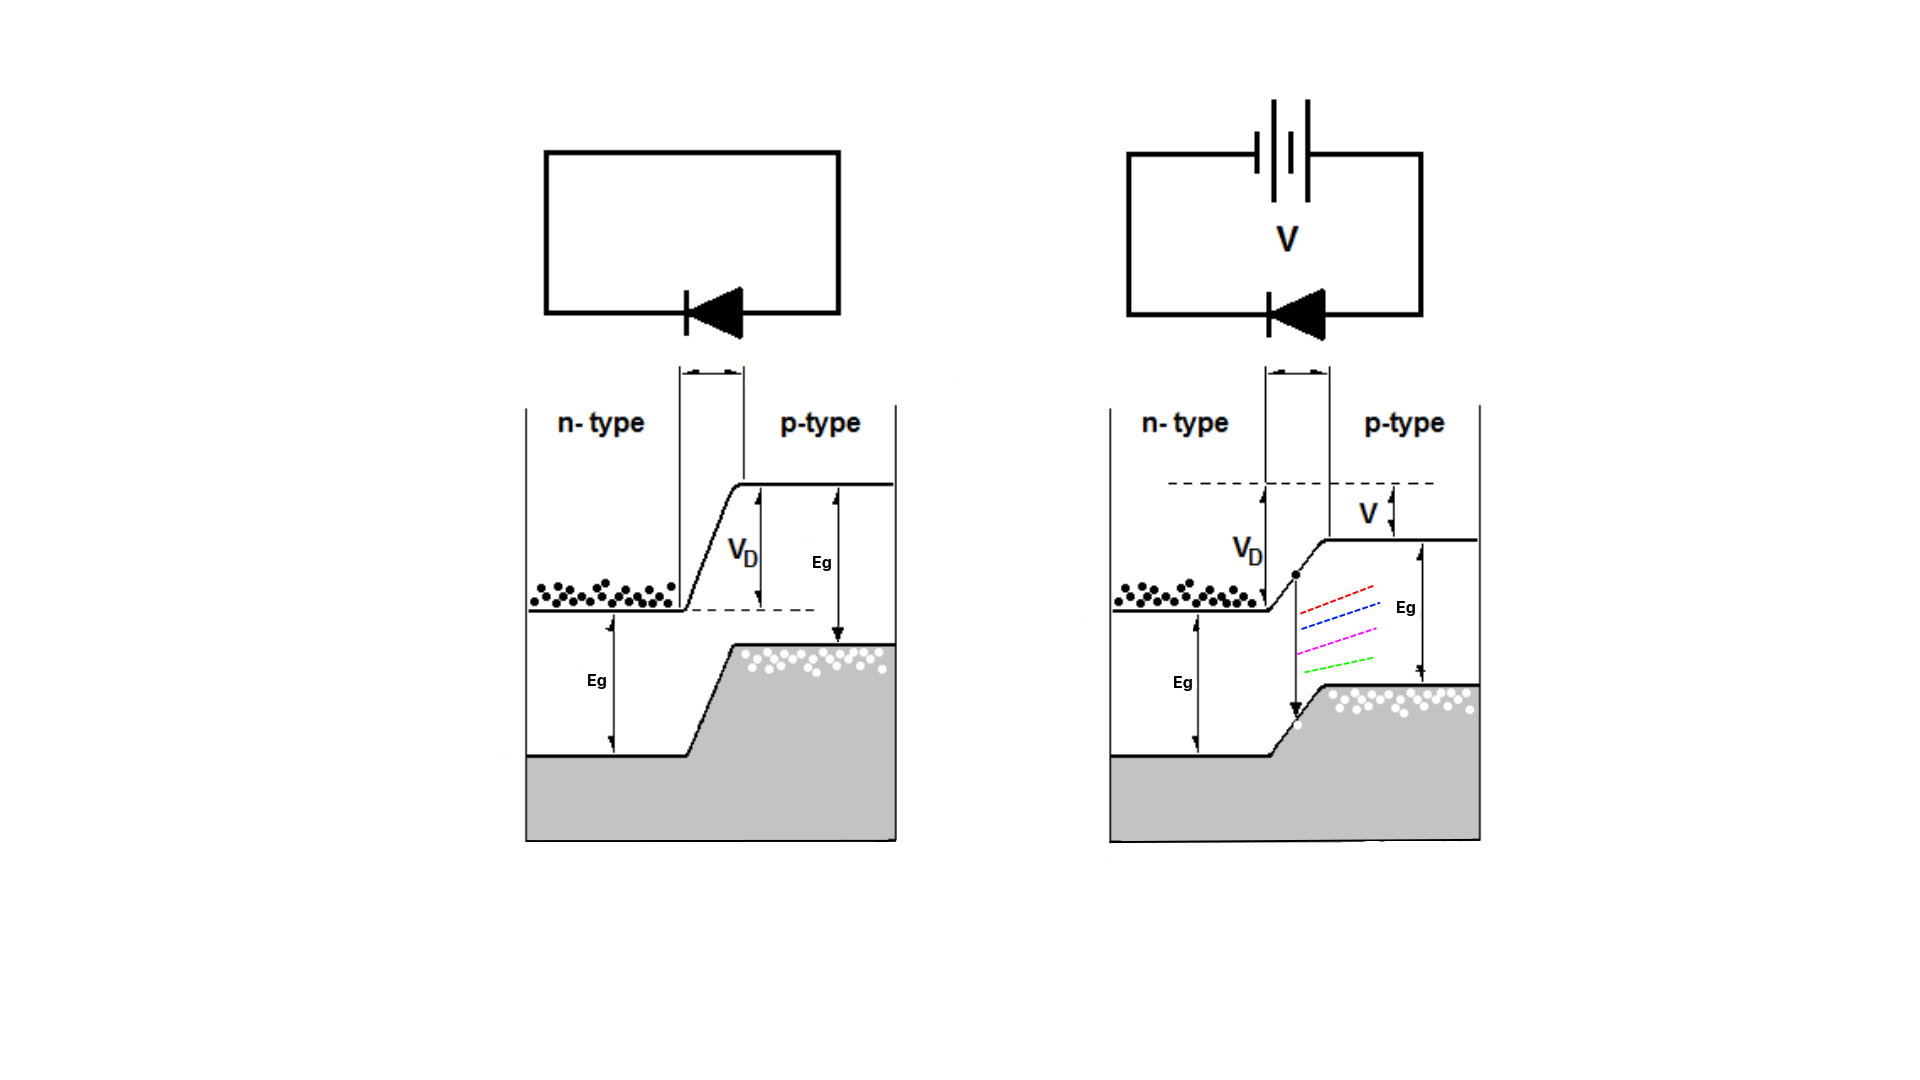
\includegraphics[width=1\textwidth]{Pictures/Other/forward_bias.png}
    \caption{Bånddiagrammet viser energien af de tilladte elektroniske tilstande gennem pn-overgangen. Den viste bøjning af lednings- og valensbåndene i overgangsområdet repræsenterer den indbyggede potentialebarriere. Ved fremadrettet bias reduceres denne barriere, så elektroner fra n-siden og huller fra p-siden lettere kan injiceres mod junctionen. Rekombination sker derfor primært nær overgangsområdet, hvor energien kan frigives som en foton.
}
    \label{fig:PN_junction_forward_bias}
\end{figure}

Ved at læse et datasheet for en LED, kan man få nyttig information som peak-bølgelængde, spektral bredde, fremadspænding, radiant flux, rise time og fall time og en række andre parametre der relaterer sig til støjniveau, præcision og optiske parametre. Der gennemgås de vigtigeste parametre relevant til dette projekt:


\begin{itemize}
    \item Fremadspænding \\ \\
    Fremadspændingen $V_f$ er den spænding, der typisk falder over LED'en ved en given forward current. LED'en drives normalt med en ønsket forward current, mens den resulterende spænding over junctionen er $V_f$.

    Fremadspændingen $V_f$ varierer mellem bølgelængder, og fremadspændingen er vidt forskellig om man vil drive en IR-LED som har en fremadspænding på $\approx$ \SI{1.3}{V}, mens at en blå LED kan have en fremadspænding på $\approx$ \SI{3.3}{V}. Forskelle i fremadspænding skyldes primært halvledermaterialets båndgab og dermed det valgte materiale. Hvor forskellige halvledere skal dopes til at få de elektriske egenskaber, som giver den bølgelængde der udsendes.

    En LED drives typisk ved at tvinge en bestemt strøm gennem komponenten ved hjælp af en strømbegrænsning, f.eks. en seriemodstand.

    \item Radiant intensitet \\ \\
    Radiant intensity angiver den udsendte optiske effekt per rumvinkel i en given retning og er derfor relevant, når man vil estimere, hvor meget lys der når en detektor placeret i en bestemt geometri. Denne parameter vises på grafer og som en del af de nøgletal i næsten ethvert datasheet for LEDer.

    \item Rise time / Fall time \\

    En LED er opbygget af to modsat dopede halvledere (n-type og p-type), hvor der omkring pn-overgangen dannes en zone uden frie ladningsbærere, kaldet "depletion layer" eller "depletion region". Denne zone adskiller ladninger på hver side af overgangen og motiverer overvejelsen for at en LED fungerer, approksimativt, som en kondensator. Dette udgår direkte fra datasheetet for LED'er, her står det ofte som "junction capacitance", denne junction, er pn-junction eller depletion regionen, denne værdi er ofte i ~10-100 pF skalaen.
    
    Ergo, ved at overveje kondensatorens egenskab om opladning og afladning af dens plader, kan man drage en parallel til LED'en, og da denne egenskab er fysisk umulig at være øjeblikkelig, er det også umuligt for en LED at tænde og slukke øjeblikkeligt. Dette udtrykkes i et datasheet som "Rise-" og "Fall time". Egenskaben er oftest symmetrisk, så:
    $$
    \text{Rise time} \approx \text{Fall time}    
    $$
    Typiske databladsværdier for LED-skiftetider ligger på en tidsskala, der er væsentligt kortere end de målevinduer, der anvendes i dette projekt. Skiftetiden bidrager derfor til en øvre grænse for, hvor hurtigt man kan multiplekse sine signaler, men er sandsynligvis ikke den begrænsende faktor i denne opstilling.
\end{itemize}

Højere kvalitets LED'er har også et eller flere lag mellem n-type og p-type, kaldet for "quantum wells" eller "multiple quantum wells" (MQW), disse forbedrer effektiviteten af en LED, og tillader for højere strømstyrke end gængse LEDer.

\section{Radiometri}
Radiometri beskriver kvantificering af elektromagnetisk stråling i fysiske enheder. Centrale radiometriske størrelser omfatter radiant flux, irradians, radians og radiant exitans \cite[s.~423]{Pedrotti2017}. I dette projekt er særligt radiant flux, irradians og responsivitet relevante. Radiant flux $\Phi_e$ beskriver den samlede optiske effekt i watt. Irradians $E_e$ beskriver den optiske effekt per areal på en overflade:
\begin{equation}
    E_e=\frac{\Phi_e}{A}.
\end{equation}
For en fotodiode med fotosensitivt areal $A_{\mathrm{PD}}$ kan den indfaldende optiske effekt tilnærmes som
\begin{equation}
    \Phi_{\mathrm{PD}}\approx E_e A_{\mathrm{PD}},
\end{equation}
hvis irradiansen antages omtrent konstant over det fotosensitive areal. Fotodiodens responsivitet $R_\lambda$ omsætter herefter den indfaldende optiske effekt til fotostrøm:
\begin{equation}
    I_{\mathrm{PD}}=R_\lambda \Phi_{\mathrm{PD}}.
\end{equation}

    \subsection{Fotodetektion}

Fotodetektion handler om at omsætte indfaldende optisk effekt til et elektrisk signal. En fotodiode absorberer fotoner og genererer en fotostrøm, som er omtrent proportional med den indfaldende optiske effekt.

En fotodiode og en LED indeholder begge en pn-overgang, men anvendes til modsatte optoelektroniske processer. I en LED omdannes elektrisk energi til lys ved rekombination, mens en fotodiode omdanner indfaldende lys til en fotostrøm ved generation og separation af elektron-hul par.

I fotovoltaisk tilstand drives fotodioden uden ekstern reverse bias. Den lysgenererede strøm opsamles typisk med en transimpedansforstærker, hvor operationsforstærkeren holder fotodiodens terminal tæt på virtuel jord. De forskellige bias-metoder for både LED og fotodiode opsummeres i tabel \ref{tab:biasering}. Hvor den fotovoltaiske tilstand er den brugte konfiguration for fotodioden i dette projekt. 

\begin{table}[h]
\centering
\caption{Sammenfatning af biaseringstilstande for LED og fotodiode.}
\label{tab:biasering}
\begin{tabularx}{\textwidth}{@{}l X X X@{}}
\toprule
 & Forward bias & Nul bias & Reverse bias \\
\midrule
LED
& Normal drift, ladningsbærere rekombinerer og udsender fotoner.
& Ingen strøm, intet lys.
& Ingen ønsket drift. Ved for høj reverse voltage kan LED'en beskadiges. \\
\addlinespace
Fotodiode
& Forward strøm dominerer over fotostrømmen. Ikke anvendelig.
& Ingen ekstern bias. I TIA-konfigurationen holdes begge terminaler omtrent ved 0 V, da katoden ligger ved virtuel jord
& Bred depletionsregion, lav kapacitans, hurtig respons men højere mørkestrøm. Kaldet for fotokonduktiv tilstand. \\
\bottomrule
\end{tabularx}
\end{table}

\begin{figure}[htbp]
    \centering
    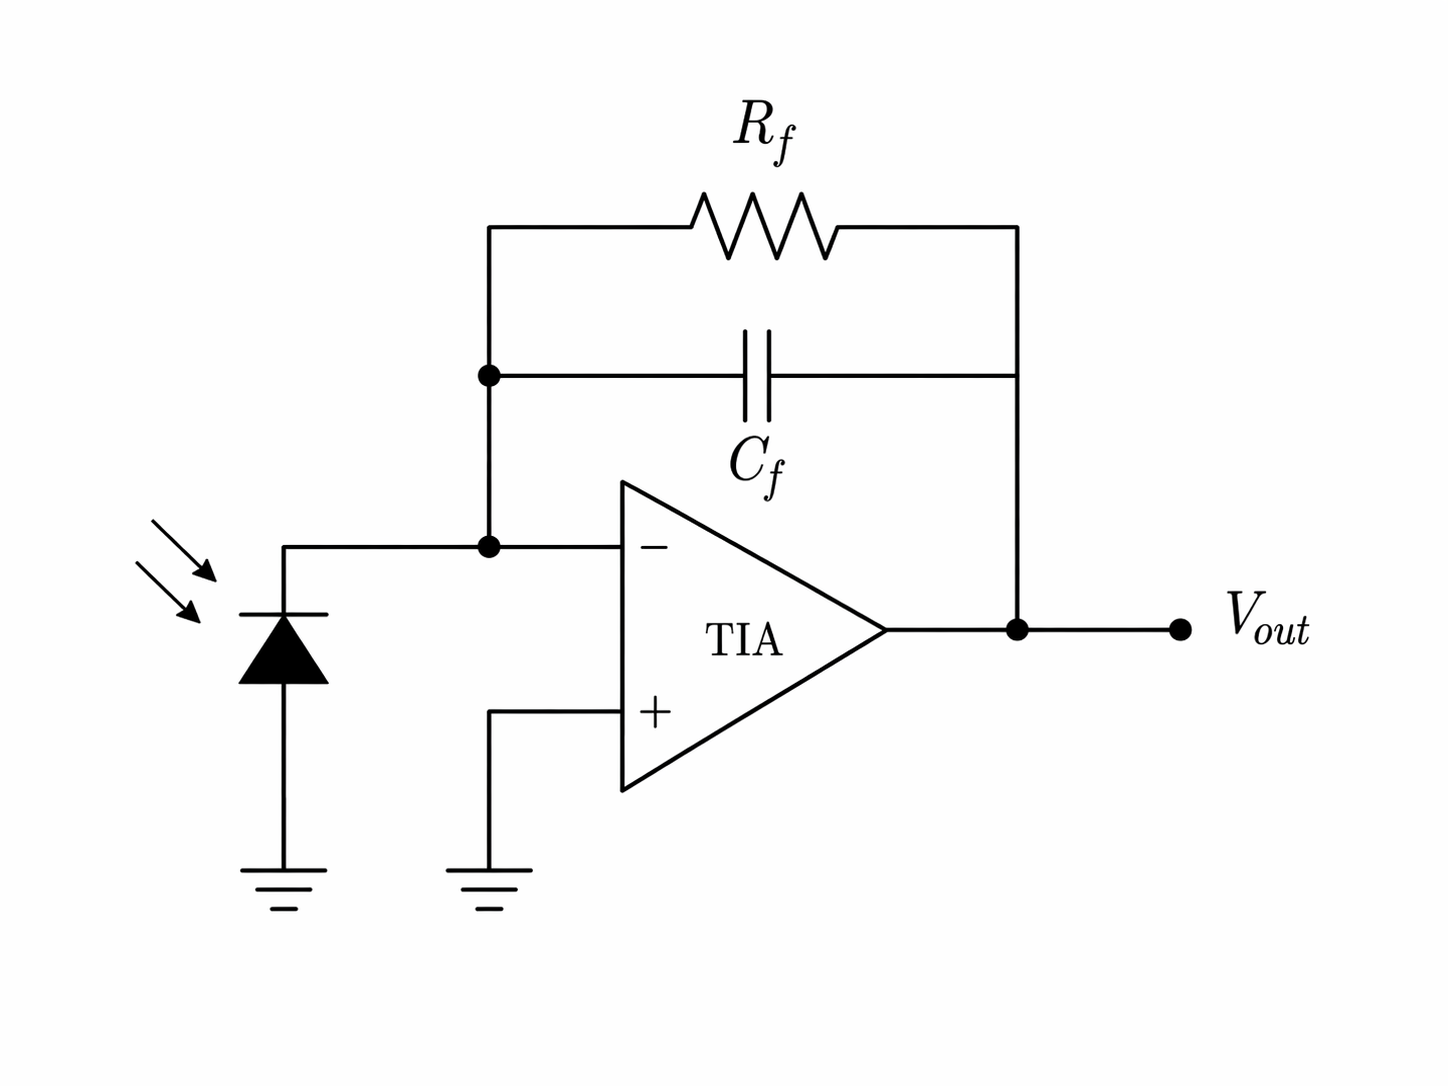
\includegraphics[width=1\textwidth]{Pictures/Other/PD photovoltaic mode.png}
    \caption{LLM-assisteret og efterfølgende manuelt redigeret illustration af en fotodiode koblet i fotovoltaisk tilstand til en transimpedansforstærker. Den viste orientering giver positiv udgangsspænding for stigende indfaldende lysintensitet.}
    \label{fig:PD_ingen_bias_TIA}
\end{figure}

Når lys rammer i eller nær depletion region i fotodioden, dannes elektron-hul par. Elektronerne drives mod n-siden (katoden), mens hullerne drives mod p-siden (anoden), dette svarer til en konventionel fotostrøm internt i fotodioden fra katode mod anode. I den anvendte TIA-konfiguration er fotodiodens anode forbundet til jord, mens katoden er forbundet til operationsforstærkerens inverterende indgang. Den lysgenererede strøm trækker derfor konventionel strøm fra summeknuden ved $−in$, gennem fotodioden og videre til GND.

Operationsforstærkeren regulerer sin udgangsspænding således, at spændingsforskellen mellem de to indgange bliver approksimativt nul, dvs. $V_- \approx V_+$. Da den ikke-inverterende indgang er jordet, holdes den inverterende indgang derfor også tæt på \SI{0}{V} (virtuel jord). Når fotodioden trækker strøm ud af summeknuden, øger operationsforstærkeren $V_{out}$, så der sendes en tilsvarende kompenserende strøm gennem feedback-modstanden $R_f$ ind i summeknuden. Herved opretholdes $V_- \approx0$, samtidig med at fotostrømmen omsættes til en udgangsspænding. 

Den fysiske fotostrøm betegnes her $I_{\text{ph}}$ og løber internt i fotodioden fra katode mod anode. I den anvendte orientering betyder det, at strøm trækkes ud af summeknuden ved op-ampens inverterende indgang. Hvis inputstrømmen til TIA'en defineres som positiv ind i summeknuden, fås derfor $I_{\mathrm{in}}=-I_{\mathrm{ph}}$. TIA'ens standardrelation er:
\begin{equation}
    V_{out}=-I_{\mathrm{in}}R_f
\end{equation}
og dermed bliver:
\begin{equation}
    V_{out}=I_{\mathrm{ph}}R_f .
\end{equation}
 Denne proces er illustreret i figur \ref{fig:PD_ingen_bias_TIA}.

Ved valg af fotodiode er særligt det aktive areal, responsiviteten, mørkestrømmen og terminalkapacitansen relevante parametre.

Herunder er en række relevante parametre:

\begin{itemize}
    \item Effektive fotosensitive areal

Det effektive fotosensitive areal er det totale brugbare areal, som en fotodiode kan opfange fotoner på. Dette område betegnes ofte som fotodiodens optiske vindue \cite[s.~388]{Pedrotti2017}. Den relevante optiske parameter for det indkommende lys er irradians:
\begin{equation}
    E_e \left[\frac{W}{\text{m}^2}\right]= \frac{P_{opt}}{A} 
\end{equation}
og med effekten isoleret:
\begin{equation}
    \Phi_{PD} \approx E_e A_{PD}
\end{equation}

    \item Responsivitet

Responsiviteten $R_{\lambda}$ angiver forholdet mellem fotostrøm og indfaldende optisk effekt ved en given bølgelængde. Den hænger sammen med fotodiodens kvanteeffektivitet, dvs. hvor stor en andel af de indfaldende fotoner der giver anledning til opsamlede ladningsbærere \cite[s.~390]{Pedrotti2017}.

\begin{equation}
    I_{PD} = R_{\lambda}\Phi_{\text{PD}}
\end{equation}
Materialerne som fotodioderne er opbygget af, har direkte effekt på responsiviteten af fotodioderne. I tabel \ref{tab:spektralrespons} ses nogle eksempler på grundstoffer og sammensatte grundstoffer som udgør størstedelen af konstruktion i fotodioder og deres typiske spektrale detektionsområde. 


\begin{table}[h]
\centering
\caption{Oversigt over detektionsområde per materiale.}
\label{tab:spektralrespons}
\begin{tabular}{ll}
\toprule
Materiale & Typisk spektralt detektionsområde $[\text{nm}]$ \\
\midrule
Silicium & 190 - 1100  \\
Germanium & 400 - 1700 \\
Indium gallium arsenide(InGaAs) & 800 - 2600  \\
\bottomrule
\end{tabular}
\end{table}

Det vises ofte på en graf hvor x-aksen repræsenterer spektralresponsen eller spændet af fotodioden i nm, og hvor y-aksen repræsenterer fotosensitiviteten fra fotodioden $\left[\frac{\text{A}}{\text{W}}\right]$.

\begin{figure}[htbp]
    \centering
    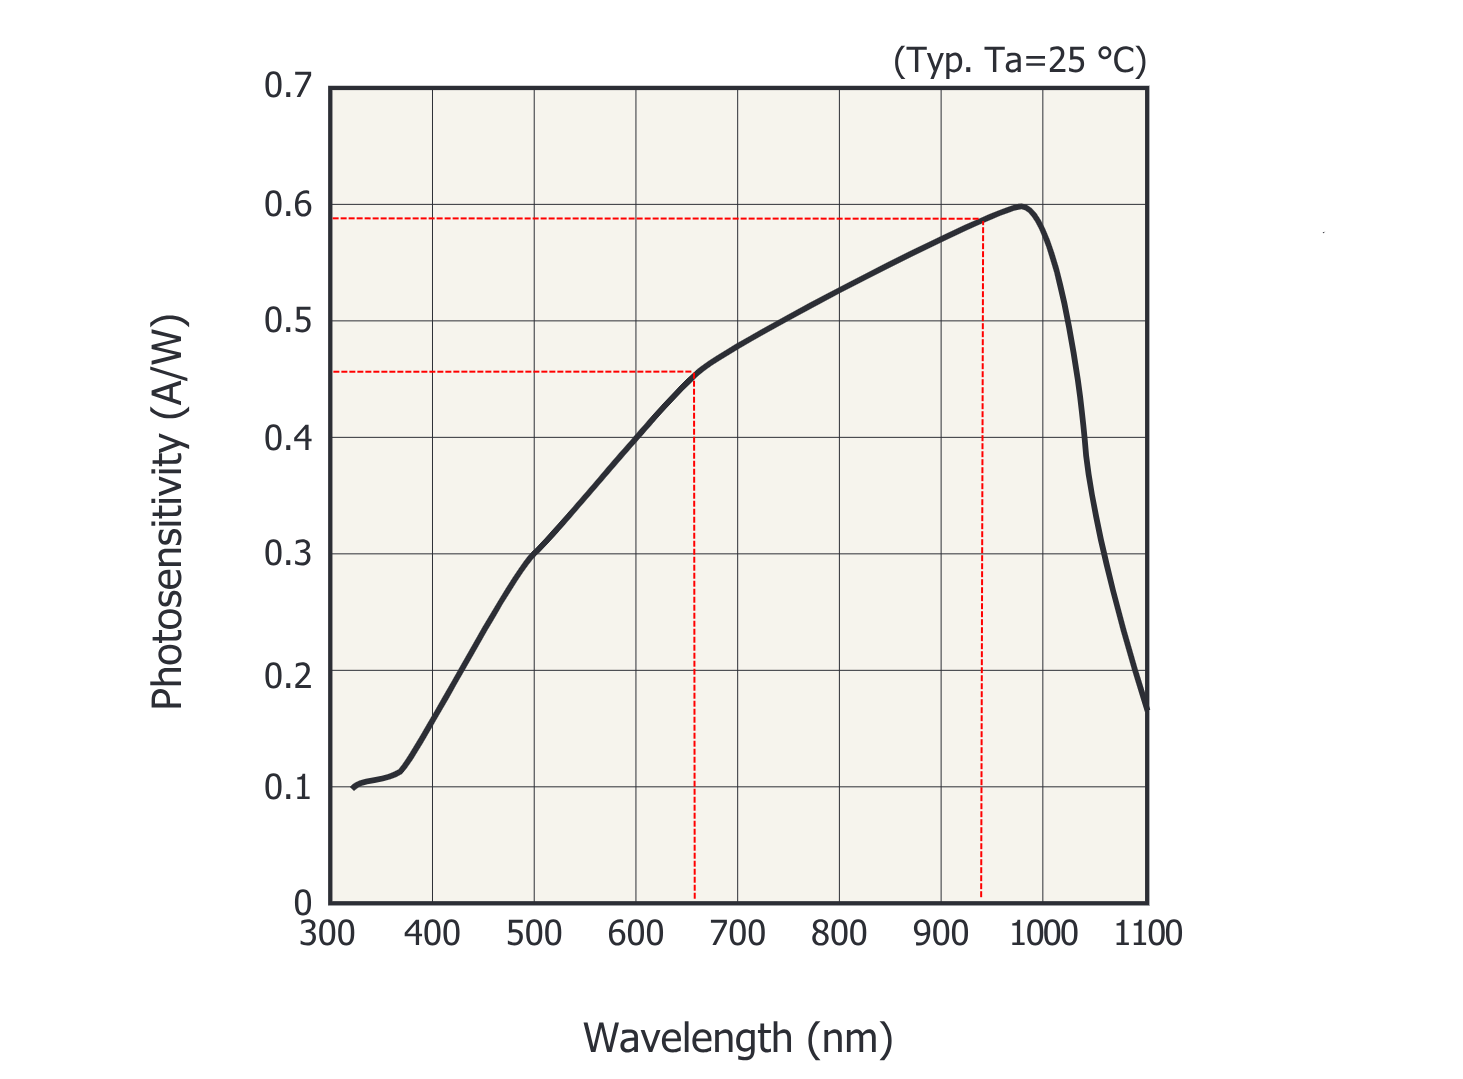
\includegraphics[width=1\textwidth]{Pictures/Datasheets/responsivitet.png}
    \caption{Responsivitet for Hamamatsu S1223 ved \SI{25}{C}. De anvendte LED-bølgelængder ved \SI{660}{nm} og \SI{940}{nm} er markeret.}
    \label{fig:responsivitet}
\end{figure}



    \item Dark Current

Mørkestrøm er den strøm, der løber i fotodioden uden belysning. Den bidrager til DC-offset og til shot noise, og den øges ved højere temperatur og reverse bias.
    
    \item Terminal kapacitans

Terminalkapacitansen påvirker TIA’ens stabilitet og båndbredde. En større kapacitans ved den inverterende indgang kan reducere fase-margenen og kræver ofte en feedback kondensator $C_f$ parallelt med $R_f$.

P-i-n-fotodioder anvender et intrinsic område mellem p- og n-regionen, hvilket kan give lavere kapacitans og hurtigere respons end en simpel pn-fotodiode \cite[s.~389]{Pedrotti2017}.

\end{itemize}


\section{Hyperspektral måling}

Hyperspektral billeddannelse registrerer en intensitet som funktion af to rumlige koordinater og bølgelængde, dvs. en datakube $I(x,y,\lambda)$ \cite{Tuchin2015}.

    \subsection{Princip}
    Princippet bag hyperspektral måling, bygger på at materialer har bølgelængdeafhængig absorption og spredning. Ved at måle $I(x,y,\lambda)$ kan man derfor undersøge, hvordan transmissionen varierer spektralt og rumligt.

    \subsection{Komponenter}
    I dette projekt blev hyperspektral information opnået sekventielt. En bredbåndet Glo-bar belyste fingeren, hvorefter det transmitterede lys blev ført gennem et lineært variabelt filter. Ved at flytte filteret med en lineær stage blev forskellige smalle spektrale bånd udvalgt og registreret med kameraet.
    
    \subsection{Sammenhæng med pulsoximetri}
    I dette projekt anvendes den hyperspektrale opstilling ikke som et fuldt pulsoximeter, men som et optisk valideringsværktøj til at undersøge den relative transmission gennem fingeren ved udvalgte bølgelængder.

    Et ideelt setup med en NIR-kilde, belyser f.eks. en finger, øre, eller anden kropsdel med blodtilførsel. Belyst væv transmitterer varierende bølgelængder, på samme måde som et analogt setup. Forskellen ligger i at med LED'er får man smalle emissionsbånd omkring udvalgte bølgelængder, mens man skal have enten filter specifikt til en bølgelængde, \SI{660}{nm} eller \SI{940}{nm} i dette tilfælde, eller man kan have prismer eller diffraktionsgittre til at isolere de ønskede bølgelængder.

    Dernæst, tager man billeder af det indfaldende lys med en bestemt frekvens, udregner pixelintensitet, filtrerer for bevægelsesstøj og finder $R$ i ratio-of-ratios, derved får man ækvivalent SpO$_2$, som ved analog måling, dog med forskellig filterkomposition.

    Dette er i det ideelle scenarie og ignorerer blandt andet varmen fra bredbåndskilden samt f.eks. prisen på NIR-følsomme kameraer.


\section{Signalbehandling}
\label{sec:signalbehandling}

\subsection{Sampling}
\label{sec:sampling}

For at digitalisere et analogt signal kræves en analog-til-digital konvertering (ADC), som sampler signalet med en fast frekvens kaldet samplingfrekvensen $f_s$. Nyquist-Shannon, eller klassisk Nyquist samplingteoremet angiver, at for at rekonstruere et signal korrekt, skal samplingfrekvensen mindst være det dobbelte af signalets højeste frekvensindhold $f_{max}$:

\begin{equation}
    f_s > 2 f_{max}
    \label{eq:nyquist}
\end{equation}

Overtrædes dette, opstår aliasing, hvor høje frekvenser fejlaflæses som lave frekvenser og forurener det rekonstruerede signal.

Det pulsatile PPG-signal følger hjertets frekvens, typisk \SIrange{0.5}{2}{Hz} svarende til 30 til 120 slag per minut \cite{Allen2007,Ruberry2025}. Systemet anvender tidsmultipleksing med tre tilstande (\SI{660}{nm}, \SI{940}{nm} og mørke), kørt med en samplingfrekvens, sat på baggrund af det brugte udstyr, f.eks. \SI{20}{kHz}. Hver kanal samples dermed med $\frac{20000}{3} \approx 6666 \ \text{Hz}$, hvilket er langt over Nyquist-grænsen for PPG-signalet og giver god tidsopløsning af pulsformen.

\subsection{Filtrering}
\label{sec:filtrering}

Den analoge signalkæde i dette system anvender filtrering til at isolere det pulsatile AC-signal fra uønskede bidrag. 

Lavpasfilteret (LPF) blev placeret efter transimpedansforstærkeren og begrænsede signalets båndbredde. Der dæmpes derfor højfrekvent støj fra omgivelserne og termisk støj, inden signalet forstærkes yderligere i efterfølgende trin.

Et højpasfilter (HPF) kan anvendes til at isolere AC-komponenten, men i dette projekt blev DC-informationen bevaret til beregning af $\frac{AC}{DC}$. Den blev designet og produceret men ikke brugt til projektet.

Det afsluttende ikke-inverterende forstærkertrin hæver signalniveauet, så ADC'ens dynamiske område udnyttes bedre.

I det digitale domæne kan signalet behandles yderligere med software-filtrering, eller ved at adskille de tre multipleksede kanaler ved at trække mørkemålingen fra de respektive LED-målinger, og kan reducere bidrag fra mørkestrøm og langsomt varierende omgivelseslys.

\subsection{Støjkilder}
\label{sec:støjkilder}

Støj i en fotodetektionskæde stammer fra flere uafhængige bidrag, som tilsammen begrænser den minimalt detekterbare effekt.

\paragraph{Fotonstøj (shot noise).} Den lysgenererede fotostrøm $I_{pd}$ består af diskrete ladningsbærere og er derfor forbundet med statistiske fluktuationer. 
Den RMS-støjstrøm er:
\begin{equation}
    i_{shot} = \sqrt{2 e I_{pd} B}
    \label{eq:shot_noise}
\end{equation}
hvor $e$ er elementarladningen og $B$ er båndbredden. Shot noise er i princippet uundgåeligt og sætter en fundamental grænse for renheden af ens signal.

\paragraph{Termisk støj (Johnson-Nyquist).} Feedback-modstanden $R_f$ i TIA'en 
genererer termisk støj med en spektral støjspænding:
\begin{equation}
    v_{Johnson} = \sqrt{4 k_B T R_f B}
    \label{eq:johnson_noise}
\end{equation}
hvor $k_B$ er Boltzmanns konstant og $T$ er temperaturen i kelvin. En høj $R_f$ giver stort gain men øger også den termiske støj.

%\paragraph{%$1/f$-støj.} Operationsforstærkere og halvlederen i fotodioden udviser støj med en spektral tæthed der stiger ved lave frekvenser. For OP27G er $1/f$-knækfrekvensen lav (ca. \SI{2.7}{Hz}), og bidraget er derved minimalt i PPG-frekvensbåndet.

%\paragraph{Omgivelseslys og 50 Hz-støj.} Elektrisk belysning moduleret ved \SI{50}{Hz} (og harmoniske) udgør en ekstern støjkilde, der kan koble ind i signalkæden. Tidsmultipleksing med subtraktion af mørkemåling undertrykker dette bidrag effektivt, da mørkemålingen registrerer omgivelseslys og mørkestrøm og trækkes fra LED-målingerne.


\section{Fejlkilder}
\label{sec:fejlkilder}

  \subsection{Bevægelsesartefakter}

Bevægelse under måling står for en betydelig del af fejlkilderne for pulsoximetri \cite{Petterson2007}. 

Artefakterne kommer især til udtryk i specifikke kliniske situationer, som f.eks. hvor patienten ufrivilligt ryster, dette kan give forkerte resultater om patientens tilstand.

Bevægelse ændrer den optiske kobling mellem LED, finger og fotodiode. Det kan ændre både DC-niveauet og den pulsatile AC-komponent uden at ændringen skyldes arteriel blodvolumen alene. Respiration kan desuden give lavfrekvent støj.
  
  \subsection{Lavt perfusionsindeks}

Perfusionsindekset (PI) er forholdet mellem AC- og DC-komponenterne i PPG-signalet, og angives ofte i procent:
\begin{equation}
    \text{PI} = \frac{AC}{DC} \cdot 100\%
    \label{eq:perfusion_index}
\end{equation}
Et lavt PI indebærer, at den pulsatile komponent er lille i forhold til den konstante absorption. Dette opstår ved perifær vasokonstriktion, f.eks. ved kulde, hypovolæmi, dvs. reduceret cirkulerende blodvolumen eller hypotension, hvor blodtilførslen til ekstremiteterne reduceres. Resultatet er et svagt og støjdomineret AC-signal, der giver et dårligt SNR og øger usikkerheden på den estimerede SpO$_2$ \cite{Webster1997,Ruberry2025}.

  \subsection{Omgivelseslys og elektromagnetisk støj}

Netspænding og elektrisk belysning kan kobles ind i det følsomme fotodiode- og TIA-kredsløb. Da fotostrømmen er lille, kan selv små indkoblede støjsignaler give synlige forstyrrelser efter forstærkning.

Da PPG-signalets AC-komponent er lille, kan indkoblet elektrisk støj blive sammenlignelig med det ønskede signal efter forstærkning. Frekvensmæssig adskillelse, analog filtrering, afskærmning og mørkesubtraktion anvendes derfor til at reducere bidraget.
  
  \subsection{Hudpigmentering og neglelak}

Melanin absorberer især i det synlige område og kan derfor påvirke den røde kanal mere end den infrarøde. Neglelak kan absorbere eller sprede lys afhængigt af farve og materiale og kan dermed ændre både DC-niveau og ratio-of-ratios \cite[s.~19]{Webster1997} \cite{Pologe2025}.

  
  \subsection{Dyshæmoglobiner}

Det klassiske to-bølgelængdeprincip antager, at hæmoglobin udelukkende eksisterer i enten iltet ($\text{HbO}_2$) eller uiltet ($\text{Hb}$) form. I praksis forekommer andre hæmoglobinformer, kaldet dyshæmoglobiner, som interfererer med målingen \cite{Webster1997,Ruberry2025}.

Kulilteforgiftning medfører dannelse af carboxyhæmoglobin (HbCO), som har en absorptionsprofil der ligner $\text{HbO}_2$ nær \SI{660}{nm}. Et pulsoximeter vil fejlaflæse HbCO som oxyhæmoglobin og dermed overestimere SpO$_2$, hvilket er klinisk kritisk \cite{Ruberry2025}.

Methæmoglobin (MetHb) har ved høje koncentrationer en tendens til at drive $R$ mod 1, svarende til SpO$_2$ $\approx$ 85\,\%, uanset den faktiske iltmætning \cite{Ruberry2025}.

Disse fejlkilder kan ikke kvantificeres pålideligt med et klassisk to-bølgelængdesystem og kræver co-oximetri med flere bølgelængder for at kvantificere de individuelle hæmoglobinformer \cite{Webster1997,Ruberry2025}.
  
  \subsection{Temperaturafhængighed af LED og fotodiode}

Temperaturen påvirker både lyskildens og detektorens egenskaber. For LED'er kan emissionsmaksimum forskydes mod længere bølgelængder med stigende junction-temperatur, i størrelsesordenen \SI{0.35}{nm} til {0.6}{nm} per celsius. En større temperaturændring kan derfor ændre de effektive ekstinktionskoefficienter og introducere en systematisk fejl i $R$ \cite[s.~66]{Webster1997}.

  \subsection{Komponenttolerancer}

Passive komponenter som modstande og kondensatorer leveres med en specificeret tolerance, typisk $\pm$1\,\% til $\pm$10\,\% for standardkomponenter. 

Tolerancerne påvirker direkte gain i transimpedansforstærkeren og knækfrekvenserne i lavpas- og højpasfilteret. En $\pm$5\,\% tolerance på $R_f$ giver en tilsvarende usikkerhed på det konverterede spændingsniveau, som akkumuleres gennem signalkæden. For Sallen-Key filtre, hvor knækfrekvensen afhænger af produktet af to modstande og to kondensatorer, kan worst-case tolerancestabling give en frekvensafvigelse som flytter knækket længere hen, eller tilbage.
